% ============================================================
%  Biodiversity & Ecosystems — Unit Booklet
%  Years 7–8  |  Victorian Curriculum F–10 Version 2.0
%  Compile with: xelatex booklet.tex  (twice for page refs)
%  Fonts: use the same ./fonts/ folder as the Forces booklet
% ============================================================
\documentclass[11pt,a4paper]{article}

% ── Fonts (compile with XeLaTeX) ─────────────────────────────────────────────
\usepackage{fontspec}
% Font path: copy the fonts/ folder from Forces/ into this Bio/ folder,
% then compile with: xelatex Bio_Ecosystems_Unit_Booklet_Yr7_8.tex
\setmainfont{Lato}[
  Path=./fonts/, Extension=.ttf, Ligatures=TeX,
  UprightFont=Lato-Regular, ItalicFont=Lato-Italic,
  BoldFont=Lato-Bold, BoldItalicFont=Lato-BoldItalic ]
\newfontfamily\headingfont{Poppins}[
  Path=./fonts/, Extension=.ttf, Ligatures=TeX,
  UprightFont=Poppins-Regular, ItalicFont=Poppins-Italic,
  BoldFont=Poppins-Bold, BoldItalicFont=Poppins-BoldItalic ]
\setlength{\headheight}{22pt}

\usepackage[protrusion=true,expansion=false]{microtype}
\usepackage[a4paper, top=2cm, bottom=2cm, left=2cm, right=2cm]{geometry}
\usepackage{xcolor}
\usepackage{tikz}
\usetikzlibrary{arrows.meta, shapes.geometric, calc, positioning,
                decorations.pathreplacing, backgrounds, patterns}
\usepackage{tcolorbox}
\tcbuselibrary{skins, breakable, raster}
\usepackage{fancyhdr}
\usepackage{titlesec}
\usepackage{enumitem}
\usepackage{booktabs}
\usepackage{tabularx}
\usepackage{array}
\usepackage{colortbl}
\usepackage{multicol}
\usepackage{amsmath}
\usepackage{needspace}
\usepackage{lastpage}
\usepackage{calc}
\usepackage{mdframed}
\usepackage{setspace}
\usepackage{ragged2e}

% ── Colour Palette ───────────────────────────────────────────────────────────
% Primary: Forest green (Bio unit identity)
\definecolor{ForestDark} {HTML}{0C2B1A}
\definecolor{Forest}     {HTML}{1E7A4E}
\definecolor{ForestLight}{HTML}{E3F5EC}
\definecolor{ForestMid}  {HTML}{2A8F5A}
% Earth / First Nations accent
\definecolor{EarthDark}  {HTML}{5E3A1A}
\definecolor{Earth}      {HTML}{8B6340}
\definecolor{EarthLight} {HTML}{F5EDE4}
% Supporting accents (carried from deck palette)
\definecolor{Teal}       {HTML}{18A999}
\definecolor{TealLight}  {HTML}{D6F3F0}
\definecolor{Amber}      {HTML}{F5A623}
\definecolor{GoldLight}  {HTML}{FFF3DC}
\definecolor{GoldDark}   {HTML}{C77F12}
\definecolor{Coral}      {HTML}{FF6B5E}
\definecolor{CoralLight} {HTML}{FFE9E6}
\definecolor{Violet}     {HTML}{7C5CE0}
\definecolor{VioletLight}{HTML}{EFE9FF}
% Neutrals
\definecolor{Ink}        {HTML}{16223A}
\definecolor{DarkGrey}   {HTML}{3A4759}
\definecolor{MidGrey}    {HTML}{AEBED4}
\definecolor{LightGrey}  {HTML}{F2F5FA}
\definecolor{Line}       {HTML}{DDE5F0}
\definecolor{Paper}      {HTML}{FBFCFE}
% Table colours
\definecolor{TableHead}  {HTML}{1E7A4E}
\definecolor{RowAlt}     {HTML}{EEF8F2}

% ── Page Style ───────────────────────────────────────────────────────────────
\pagestyle{fancy}
\fancyhf{}
\renewcommand{\headrulewidth}{0.4pt}
\renewcommand{\headrule}{\hbox to\headwidth{\color{Forest}\leaders\hrule height \headrulewidth\hfill}}
\fancyhead[L]{\headingfont\small\color{Forest}Biodiversity \& Ecosystems}
\fancyhead[R]{\headingfont\small\color{DarkGrey}Years 7--8 \textbar{} Victorian Curriculum F--10 v2.0}
\fancyfoot[C]{\headingfont\small\color{DarkGrey}\thepage\ \textbar{} \pageref{LastPage}}
\fancypagestyle{plain}{%
  \fancyhf{}
  \fancyfoot[C]{\headingfont\small\color{DarkGrey}\thepage\ \textbar{} \pageref{LastPage}}
  \renewcommand{\headrulewidth}{0pt}
}

% ── Section Formatting ───────────────────────────────────────────────────────
\titleformat{\section}
  {\headingfont\color{Forest}\Large\bfseries}
  {}{0em}{}
  [{\color{Teal}\rule[0.6ex]{2.2em}{3pt}}{\color{Line}\rule[0.6ex]{\dimexpr\linewidth-2.2em\relax}{1pt}}]
\titlespacing{\section}{0pt}{18pt}{8pt}

\titleformat{\subsection}
  {\headingfont\color{ForestMid}\large\bfseries}
  {\thesubsection}{0.6em}{}
\titlespacing{\subsection}{0pt}{12pt}{4pt}

\titleformat{\subsubsection}
  {\headingfont\color{Forest}\normalsize\bfseries}
  {}{0em}{}
\titlespacing{\subsubsection}{0pt}{8pt}{2pt}

% Kicker / eyebrow label
\newcommand{\kicker}[2][Teal]{%
  {\headingfont\bfseries\footnotesize\color{#1}%
   \textcolor{#1}{\rule[0.18ex]{1.6em}{2.2pt}}\hspace{0.5em}\MakeUppercase{#2}\par}%
  \vspace{2pt}}

% ── Custom tcolorbox Environments ────────────────────────────────────────────

% Section divider banner (forest green)
\newcommand{\sectiondiv}[3]{%
  \needspace{5\baselineskip}
  \begin{tcolorbox}[
    enhanced, breakable=false, arc=3.5mm,
    colback=ForestDark, colframe=ForestDark, boxrule=0pt,
    sidebyside, sidebyside align=center,
    lefthand width=2.0cm,
    left=2mm, right=4mm, top=4mm, bottom=4mm
  ]
    \begin{center}
      {\headingfont\bfseries\color{Forest!35!ForestDark}\fontsize{50}{50}\selectfont #1}
    \end{center}
    \tcblower
    {\headingfont\bfseries\color{white}\LARGE #2}\\[3pt]
    {\itshape\color{white!75!ForestDark}\small #3}
  \end{tcolorbox}%
}

% Key info box (forest green)
\newtcolorbox{infobox}[1]{
  breakable, arc=2.5mm, boxrule=0.5pt,
  colback=ForestLight, colframe=Forest!40,
  fonttitle=\headingfont\bfseries, coltitle=ForestMid,
  title={#1},
  left=4mm, right=3.5mm, top=2.5mm, bottom=2.5mm
}

% First Nations callout (earth brown)
\newtcolorbox{fnbox}[1]{
  breakable, arc=2.5mm, boxrule=0.5pt,
  colback=EarthLight, colframe=Earth!40,
  fonttitle=\headingfont\bfseries, coltitle=EarthDark,
  title={#1},
  left=4mm, right=3.5mm, top=2.5mm, bottom=2.5mm
}

% Scaffold box (amber / yellow)
\newtcolorbox{scaffold}[1]{
  breakable, arc=2.5mm, boxrule=0.5pt,
  colback=GoldLight, colframe=Amber!40,
  fonttitle=\headingfont\bfseries, coltitle=GoldDark,
  title={#1},
  left=4mm, right=3.5mm, top=2.5mm, bottom=2.5mm
}

% Worked example box
\newtcolorbox{workedex}[1]{
  breakable, arc=2.5mm, boxrule=0.5pt,
  colback=white, colframe=Amber!50,
  fonttitle=\headingfont\bfseries, coltitle=GoldDark,
  title={#1},
  left=4mm, right=3.5mm, top=2.5mm, bottom=2.5mm
}

% Year 7 box (forest green)
\newtcolorbox{yr7box}{
  breakable, arc=2.5mm, boxrule=0.5pt,
  colback=ForestLight, colframe=Forest!40,
  left=4mm, right=3.5mm, top=2.5mm, bottom=2.5mm
}

% Year 8 extension box (violet)
\newtcolorbox{yr8box}{
  breakable, arc=2.5mm, boxrule=0.5pt,
  colback=VioletLight, colframe=Violet!40,
  left=4mm, right=3.5mm, top=2.5mm, bottom=2.5mm
}

% ── Custom Commands ───────────────────────────────────────────────────────────

% Answer box
\newcommand{\answerbox}[1]{%
  \begin{tcolorbox}[
    enhanced, breakable, arc=2mm,
    colback=Paper, colframe=Line,
    left=2mm, right=2mm, top=1mm, bottom=1mm,
    boxrule=1pt,
    height=#1
  ]
  \end{tcolorbox}%
}

% Question command
\newcommand{\question}[3]{%
  \needspace{3\baselineskip}%
  \medskip
  \noindent\textbf{Q#1}\ifx&#2&\else\ \textcolor{DarkGrey}{(#2 mark\ifnum#2=1\else s\fi)}\fi\quad #3%
  \medskip
}

% Marks note
\newcommand{\markscount}[1]{\hfill\textcolor{DarkGrey}{\textit{(#1 mark\ifnum#1=1\else s\fi)}}}

% Figure caption
\newcommand{\figcap}[1]{%
  \begin{center}
    \small\itshape\color{DarkGrey} #1
  \end{center}%
}

% Table column types
\newcolumntype{L}[1]{>{\RaggedRight\arraybackslash}p{#1}}
\newcolumntype{C}[1]{>{\Centering\arraybackslash}p{#1}}

% Table header
\newcommand{\thead}[1]{\cellcolor{TableHead}\color{white}\bfseries #1}
\newcommand{\talt}{\rowcolor{RowAlt}}
\newcommand{\tmid}{\rowcolor{MidGrey}}

% Answer lines
\newcommand{\anslines}[1]{%
  \vspace{2pt}%
  \foreach \n in {1,...,#1}{%
    \par\noindent\rule{\linewidth}{0.3pt}\vspace{3pt}%
  }%
}

% ── TikZ Diagram Macros ───────────────────────────────────────────────────────

\tikzset{
  bio arrow/.style={-{Stealth[length=6pt,width=4pt]}, line width=1.8pt},
  thin bio/.style={-{Stealth[length=5pt,width=3.5pt]}, line width=1.2pt},
}

% D1: MRS GREN spider diagram
\newcommand{\diagMrsGren}{%
\begin{center}
\begin{tikzpicture}[font=\small]
  % Centre circle
  \node[draw=Forest, fill=ForestLight, circle, minimum size=2.2cm,
        font=\small\bfseries, text=Forest, align=center]
        (centre) at (0,0) {MRS\\GREN};
  % 7 satellite nodes, evenly spaced
  \node[draw=Teal, fill=TealLight, rounded corners=4pt,
        minimum width=2.8cm, minimum height=0.9cm,
        font=\small\bfseries, text=Ink, align=center] (M) at (0, 3.2) {\textbf{M}ovement};
  \node[draw=Teal, fill=TealLight, rounded corners=4pt,
        minimum width=2.8cm, minimum height=0.9cm,
        font=\small\bfseries, text=Ink, align=center] (R1) at (2.9, 2.0) {\textbf{R}espiration};
  \node[draw=Teal, fill=TealLight, rounded corners=4pt,
        minimum width=2.8cm, minimum height=0.9cm,
        font=\small\bfseries, text=Ink, align=center] (S) at (3.2, -0.3) {\textbf{S}ensitivity};
  \node[draw=Teal, fill=TealLight, rounded corners=4pt,
        minimum width=2.8cm, minimum height=0.9cm,
        font=\small\bfseries, text=Ink, align=center] (G) at (2.0, -2.4) {\textbf{G}rowth};
  \node[draw=Teal, fill=TealLight, rounded corners=4pt,
        minimum width=2.8cm, minimum height=0.9cm,
        font=\small\bfseries, text=Ink, align=center] (R2) at (-2.0, -2.4) {\textbf{R}eproduction};
  \node[draw=Teal, fill=TealLight, rounded corners=4pt,
        minimum width=2.8cm, minimum height=0.9cm,
        font=\small\bfseries, text=Ink, align=center] (E) at (-3.2, -0.3) {\textbf{E}xcretion};
  \node[draw=Teal, fill=TealLight, rounded corners=4pt,
        minimum width=2.8cm, minimum height=0.9cm,
        font=\small\bfseries, text=Ink, align=center] (N) at (-2.9, 2.0) {\textbf{N}utrition};
  % Lines from centre
  \foreach \nd in {M, R1, S, G, R2, E, N}
    \draw[thick, Forest!50] (centre) -- (\nd);
\end{tikzpicture}
\end{center}}

% D2: Linnaean funnel (7 levels) — explicit trapezoids, no pgf array tricks
\newcommand{\diagLinnaean}{%
\begin{center}
\begin{tikzpicture}[font=\small]
  % Each trapezoid: fill, then label. Widths narrow from 8 to 2 cm; step 0.65 cm/level.
  \fill[Forest!80!white, draw=white, line width=0pt]  (-4.0,0.00) -- (4.0,0.00) -- (3.5,-0.60) -- (-3.5,-0.60) -- cycle;
  \node[font=\small\bfseries, text=ForestDark] at (0,-0.30) {Kingdom};
  \fill[Forest!70!white, draw=white, line width=0pt]  (-3.5,-0.65) -- (3.5,-0.65) -- (3.0,-1.25) -- (-3.0,-1.25) -- cycle;
  \node[font=\small\bfseries, text=ForestDark] at (0,-0.95) {Phylum};
  \fill[Forest!60!white, draw=white, line width=0pt]  (-3.0,-1.30) -- (3.0,-1.30) -- (2.5,-1.90) -- (-2.5,-1.90) -- cycle;
  \node[font=\small\bfseries, text=ForestDark] at (0,-1.60) {Class};
  \fill[Forest!50!white, draw=white, line width=0pt]  (-2.5,-1.95) -- (2.5,-1.95) -- (2.0,-2.55) -- (-2.0,-2.55) -- cycle;
  \node[font=\small\bfseries, text=ForestDark] at (0,-2.25) {Order};
  \fill[Teal!55!white, draw=white, line width=0pt]    (-2.0,-2.60) -- (2.0,-2.60) -- (1.5,-3.20) -- (-1.5,-3.20) -- cycle;
  \node[font=\small\bfseries, text=ForestDark] at (0,-2.90) {Family};
  \fill[Teal!70!white, draw=white, line width=0pt]    (-1.5,-3.25) -- (1.5,-3.25) -- (1.0,-3.85) -- (-1.0,-3.85) -- cycle;
  \node[font=\small\bfseries, text=ForestDark] at (0,-3.55) {Genus};
  \fill[Teal!85!white, draw=white, line width=0pt]    (-1.0,-3.90) -- (1.0,-3.90) -- (0.5,-4.50) -- (-0.5,-4.50) -- cycle;
  \node[font=\small\bfseries, text=ForestDark] at (0,-4.20) {Species};
  % Annotations
  \node[font=\scriptsize\itshape, text=DarkGrey, anchor=west] at (4.2, 0.0)  {broadest (most general)};
  \node[font=\scriptsize\itshape, text=DarkGrey, anchor=west] at (0.7,-4.5) {most specific};
  \draw[-{Stealth[length=5pt]}, DarkGrey!60, thick] (4.0,0.0) -- (4.0,-4.4);
  \node[font=\scriptsize\itshape, text=DarkGrey, rotate=90, anchor=south] at (4.6,-2.2)
    {increasing specificity};
\end{tikzpicture}
\end{center}}

% D3: Six Kingdoms grid — fully explicit options on every node (no named style)
% text width=3.8cm guarantees paragraph mode so \\ line breaks work
\newcommand{\diagSixKingdoms}{%
\begin{center}
\begin{tikzpicture}[font=\small]
  % Top row: Eukaryotes
  \node[draw=Forest!70, fill=Forest!25!white, rounded corners=5pt,
        line width=1pt, align=center, text width=3.8cm,
        inner sep=6pt, minimum height=2.6cm]
    at (-4.6, 0) {\textbf{Animalia}\\{\scriptsize Humans, kangaroos, insects, fish}};
  \node[draw=Forest!70, fill=Forest!18!white, rounded corners=5pt,
        line width=1pt, align=center, text width=3.8cm,
        inner sep=6pt, minimum height=2.6cm]
    at (0, 0) {\textbf{Plantae}\\{\scriptsize Wattles, grass, ferns, mosses}};
  \node[draw=Forest!70, fill=Forest!12!white, rounded corners=5pt,
        line width=1pt, align=center, text width=3.8cm,
        inner sep=6pt, minimum height=2.6cm]
    at (4.6, 0) {\textbf{Fungi}\\{\scriptsize Mushrooms, moulds, yeasts}};
  % Bottom row: prokaryotes + Protista
  \node[draw=Forest!70, fill=Teal!18!white, rounded corners=5pt,
        line width=1pt, align=center, text width=3.8cm,
        inner sep=6pt, minimum height=2.6cm]
    at (-4.6, -3.2) {\textbf{Protista}\\{\scriptsize Amoeba, algae, paramecium}};
  \node[draw=Forest!70, fill=Teal!12!white, rounded corners=5pt,
        line width=1pt, align=center, text width=3.8cm,
        inner sep=6pt, minimum height=2.6cm]
    at (0, -3.2) {\textbf{Bacteria}\\{\scriptsize \textit{E.~coli,} \textit{Salmonella}}};
  \node[draw=Forest!70, fill=Teal!8!white, rounded corners=5pt,
        line width=1pt, align=center, text width=3.8cm,
        inner sep=6pt, minimum height=2.6cm]
    at (4.6, -3.2) {\textbf{Archaea}\\{\scriptsize Hot spring microbes}};
  % Row labels
  \node[font=\scriptsize\itshape, text=DarkGrey, anchor=east]
    at (-7.0,  0.0) {Eukaryotes};
  \node[font=\scriptsize\itshape, text=DarkGrey, anchor=east]
    at (8.5, -3.2) {Prokaryotes};
  \draw[DarkGrey!50, dashed] (-2.3,-1.6) -- (6.9,-1.6);
  \draw[DarkGrey!50, dashed] (-2.3,-4.6) -- (-2.3,-1.6);
\end{tikzpicture}
\end{center}}

% D4: Simple dichotomous key flowchart (4 organisms)
\newcommand{\diagDichotKey}{%
\begin{center}
\begin{tikzpicture}[font=\small,
    question/.style={draw=Forest, fill=ForestLight, rounded corners=4pt,
                     align=center, inner sep=4pt, minimum width=5.5cm},
    result/.style={draw=Teal, fill=TealLight, rounded corners=4pt,
                   align=center, inner sep=3pt, minimum width=3.5cm}]
  % Nodes
  \node[question] (q1) at (0,0) {Does it have a backbone?};
  \node[question] (q2) at (-4.2,-2.2) {Does it have 4 legs?};
  \node[question] (q3) at (4.2,-2.2) {Does it have 6 legs?};
  \node[result]   (r1) at (-6.3,-4.4) {Eastern grey\\kangaroo};
  \node[result]   (r2) at (-2.1,-4.4) {Eastern brown\\snake};
  \node[result]   (r3) at (2.1,-4.4) {Common\\grasshopper};
  \node[result]   (r4) at (6.3,-4.4) {Garden\\orb-weaver spider};
  % Arrows — all originate from south (bottom-centre) of each node
  \draw[bio arrow, Forest] (q1.south) -- node[above, sloped, font=\scriptsize]{Yes} (q2.north);
  \draw[bio arrow, Coral]  (q1.south) -- node[above, sloped, font=\scriptsize]{No}  (q3.north);
  \draw[bio arrow, Forest] (q2.south) -- node[above, sloped, font=\scriptsize]{Yes} (r1.north);
  \draw[bio arrow, Coral]  (q2.south) -- node[above, sloped, font=\scriptsize]{No}  (r2.north);
  \draw[bio arrow, Forest] (q3.south) -- node[above, sloped, font=\scriptsize]{Yes} (r3.north);
  \draw[bio arrow, Coral]  (q3.south) -- node[above, sloped, font=\scriptsize]{No}  (r4.north);
\end{tikzpicture}
\end{center}}

% D5: Ecosystem biotic/abiotic diagram
\newcommand{\diagEcosystem}{%
\begin{center}
\begin{tikzpicture}[font=\small]
  % Two overlapping-style boxes
  \node[draw=Forest, fill=ForestLight, rounded corners=6pt,
        minimum width=6.5cm, minimum height=5.5cm] (bio) at (-3.5,0) {};
  \node[draw=Teal, fill=TealLight, rounded corners=6pt,
        minimum width=6.5cm, minimum height=5.5cm] (abio) at (3.5,0) {};
  \node[font=\normalsize\bfseries, text=Forest] at (-3.5, 2.4) {Biotic factors};
  \node[font=\scriptsize\itshape, text=DarkGrey] at (-3.5, 1.9) {(living components)};
  \node[font=\small, text=Ink, align=center] at (-3.5, 0.8) {Plants \& trees};
  \node[font=\small, text=Ink, align=center] at (-3.5, 0.2) {Animals};
  \node[font=\small, text=Ink, align=center] at (-3.5,-0.4) {Fungi \& bacteria};
  \node[font=\small, text=Ink, align=center] at (-3.5,-1.0) {Algae};
  \node[font=\small, text=Ink, align=center] at (-3.5,-1.6) {Dead organic matter};
  \node[font=\normalsize\bfseries, text=Teal] at (3.5, 2.4) {Abiotic factors};
  \node[font=\scriptsize\itshape, text=DarkGrey] at (3.5, 1.9) {(non-living components)};
  \node[font=\small, text=Ink, align=center] at (3.5, 0.8) {Sunlight};
  \node[font=\small, text=Ink, align=center] at (3.5, 0.2) {Temperature};
  \node[font=\small, text=Ink, align=center] at (3.5,-0.4) {Water \& rainfall};
  \node[font=\small, text=Ink, align=center] at (3.5,-1.0) {Soil nutrients};
  \node[font=\small, text=Ink, align=center] at (3.5,-1.6) {Wind \& altitude};
  % Centre label
  \node[draw=GoldDark, fill=GoldLight, rounded corners=3pt,
        font=\small\bfseries, text=GoldDark, inner sep=4pt, align=center]
        at (0,0) {ECOSYSTEM\\{\scriptsize\color{DarkGrey}(biotic + abiotic)}};
\end{tikzpicture}
\end{center}}

% D6: Simple food web (Victorian woodland, 5 nodes)
\newcommand{\diagFoodWeb}{%
\begin{center}
\begin{tikzpicture}[font=\small,
    prod/.style={draw=Forest, fill=ForestLight, rounded corners=4pt,
                 align=center, inner sep=3pt, minimum width=2.8cm},
    cons1/.style={draw=Amber, fill=GoldLight, rounded corners=4pt,
                  align=center, inner sep=3pt, minimum width=2.8cm},
    cons2/.style={draw=Coral, fill=CoralLight, rounded corners=4pt,
                  align=center, inner sep=3pt, minimum width=2.8cm},
    apex/.style={draw=Violet, fill=VioletLight, rounded corners=4pt,
                 align=center, inner sep=3pt, minimum width=3.2cm}]
  % Nodes
  \node[prod]  (grass)  at (-3.0, -3.5) {Wallaby grass};
  \node[prod]  (wattle) at (3.0,  -3.5) {Wattle seeds};
  \node[cons1] (roo)    at (-4.5, -1.8) {Kangaroo};
  \node[cons1] (grass2) at (0,    -1.8) {Grasshopper};
  \node[cons1] (rosella)at (4.5,  -1.8) {Crimson rosella};
  \node[cons2] (falcon) at (-2.0,  0.0) {Brown falcon};
  \node[cons2] (monitor)at (3.0,   0.0) {Lace monitor};
  \node[apex]  (eagle)  at (0.5,   1.8) {Wedge-tailed eagle};
  % Arrows (energy flow)
  \draw[bio arrow, DarkGrey!60] (grass)  -- (roo);
  \draw[bio arrow, DarkGrey!60] (grass)  -- (grass2);
  \draw[bio arrow, DarkGrey!60] (wattle) -- (rosella);
  \draw[bio arrow, DarkGrey!60] (wattle) -- (grass2);
  \draw[bio arrow, DarkGrey!60] (roo)    -- (falcon);
  \draw[bio arrow, DarkGrey!60] (grass2) -- (falcon);
  \draw[bio arrow, DarkGrey!60] (grass2) -- (monitor);
  \draw[bio arrow, DarkGrey!60] (rosella)-- (monitor);
  \draw[bio arrow, DarkGrey!60] (falcon) -- (eagle);
  \draw[bio arrow, DarkGrey!60] (monitor)-- (eagle);
  % Labels
  \node[font=\scriptsize\itshape, text=Forest,  anchor=east] at (-5.5,-3.5) {Producers};
  \node[font=\scriptsize\itshape, text=GoldDark, anchor=east] at (-6,-1.8) {1\textsuperscript{ry} consumers};
  \node[font=\scriptsize\itshape, text=Coral,   anchor=east] at (-6, 0.0) {2\textsuperscript{ry} consumers};
  \node[font=\scriptsize\itshape, text=Violet,  anchor=east] at (-5.5, 1.8) {Apex};
\end{tikzpicture}
\end{center}}

% D7: Adaptation types — 3 explicit boxes, no foreach with special chars
\newcommand{\diagAdaptations}{%
\begin{center}
\begin{tikzpicture}[font=\small]
  % Structural
  \fill[Forest!20, draw=Forest!70, rounded corners=6pt, line width=1.5pt]
    (-7.5, 0.4) rectangle (-2.5, -3.2);
  \node[font=\normalsize\bfseries, text=Forest!80!black] at (-5.0, 0.0) {Structural};
  \node[font=\small, text=Ink, align=center] at (-5.0, -1.4)
    {Body features:\\[2pt]thick fur, webbed feet,\\spines, camouflage};
  % Behavioural
  \fill[Teal!20, draw=Teal!70, rounded corners=6pt, line width=1.5pt]
    (-2.0, 0.4) rectangle (3.0, -3.2);
  \node[font=\normalsize\bfseries, text=Teal!80!black] at (0.5, 0.0) {Behavioural};
  \node[font=\small, text=Ink, align=center] at (0.5, -1.4)
    {Actions:\\[2pt]hibernation, migration,\\nocturnal activity};
  % Physiological
  \fill[Violet!20, draw=Violet!70, rounded corners=6pt, line width=1.5pt]
    (3.5, 0.4) rectangle (8.5, -3.2);
  \node[font=\normalsize\bfseries, text=Violet!80!black] at (6.0, 0.0) {Physiological};
  \node[font=\small, text=Ink, align=center] at (6.0, -1.4)
    {Internal processes:\\[2pt]concentrated urine,\\reduced heart rate};
\end{tikzpicture}
\end{center}}

% ── Document ──────────────────────────────────────────────────────────────────
\begin{document}
\setlength{\parindent}{0pt}
\setlength{\parskip}{4pt}

% ══════════════════════════════════════════════════════════════════════════════
%  COVER PAGE
% ══════════════════════════════════════════════════════════════════════════════
\thispagestyle{plain}

\begin{tcolorbox}[
  enhanced, breakable=false, arc=4mm,
  colback=ForestDark, colframe=ForestDark,
  left=6mm, right=6mm, top=9mm, bottom=9mm,
  boxrule=0pt
]
  \begin{center}
    {\headingfont\bfseries\color{Teal}\footnotesize\MakeUppercase{Unit Booklet \textbullet\ Years 7 and 8}}\\[10pt]
    {\headingfont\bfseries\color{white}\fontsize{36}{40}\selectfont Biodiversity \& Ecosystems}\\[8pt]
    {\large\color{white!85!ForestDark}\itshape Classification \textbullet\ Food webs \textbullet\ Adaptations \textbullet\ Conservation}\\[14pt]
    {\headingfont\color{white!72!ForestDark}\normalsize
      Victorian Curriculum F--10 Version 2.0 \textbar{}
      VCSSU091 \textbar{} VCSSU093 \textbar{} VCSIS108--113}
  \end{center}
\end{tcolorbox}

\vspace{10pt}

% Student details
\begin{tabular}{@{}p{3.5cm} p{6cm} p{2cm} p{3.5cm}@{}}
  \textbf{Name:}    & \underline{\hspace{5.8cm}} & \textbf{Class:}      & \underline{\hspace{3.3cm}} \\[8pt]
  \textbf{Teacher:} & \underline{\hspace{5.8cm}} & \textbf{Year level:} & \underline{\hspace{3.3cm}} \\
\end{tabular}

\vspace{10pt}

\begin{fnbox}{Acknowledgement of Country}
This booklet was created on the unceded Country of the Wurundjeri-Woiwurrung people of the Kulin Nation. We acknowledge Elders past, present, and emerging, and recognise that First Nations peoples have cared for this Country and its biodiversity for tens of thousands of years. Throughout this unit we will explore how Wurundjeri-Woiwurrung ecological knowledge connects to, and enriches, scientific understanding of biodiversity and ecosystems.
\end{fnbox}

\vspace{8pt}

\begin{infobox}{How to use this booklet}
This booklet covers the full Biodiversity \& Ecosystems unit. Work through it in order --- each section builds on the last.

\medskip
\begin{tabular}{@{}ll@{}}
  \textcolor{Forest}{\rule{10pt}{10pt}}\ \textbf{Green boxes}  & Year 7 core content and questions \\
  \textcolor{Violet}{\rule{10pt}{10pt}}\ \textbf{Purple boxes} & Year 8 extension tasks \\
  \textcolor{GoldDark}{\rule{10pt}{10pt}}\ \textbf{Yellow boxes} & Scaffolds and worked examples \\
  \textcolor{Earth}{\rule{10pt}{10pt}}\ \textbf{Brown boxes}   & First Nations perspectives \\
\end{tabular}
\end{infobox}

\vspace{8pt}

% Contents table
\begin{tabular}{@{}C{0.6cm} L{9cm} C{1.8cm} C{1.8cm}@{}}
  \thead{\#} & \thead{Section} & \thead{Yr 7} & \thead{Yr 8} \\
  \talt 1  & Living or Non-living? (MRS GREN) & p.\ 2 & p.\ 4 \\
         2  & Classification --- Linnaean Levels & p.\ 5 & p.\ 7 \\
  \talt  3  & Scientific Names \& The Six Kingdoms & p.\ 8 & p.\ 11 \\
         4  & Dichotomous Keys & p.\ 12 & p.\ 15 \\
  \talt  5  & Australian Ecosystems \& Biodiversity & p.\ 16 & p.\ 19 \\
         6  & Food Webs \& Energy Flow & p.\ 20 & p.\ 23 \\
  \talt  7  & Ecosystem Services & p.\ 24 & p.\ 27 \\
         8  & Adaptations & p.\ 28 & p.\ 31 \\
  \talt  9  & Introduced Species & p.\ 32 & p.\ 35 \\
        10  & Human Impacts on Ecosystems & p.\ 36 & p.\ 39 \\
  \talt 11  & Conservation \& Action & p.\ 40 & p.\ 43 \\
\end{tabular}

\newpage

% ══════════════════════════════════════════════════════════════════════════════
%  SECTION 1 — LIVING OR NON-LIVING?
% ══════════════════════════════════════════════════════════════════════════════
\sectiondiv{1}{Living or Non-living?}{MRS GREN \textbullet{} Seven life processes \textbullet{} Dead vs non-living}

\subsection{What makes something alive?}

Scientists use seven characteristics to define life. These are remembered using the mnemonic \textbf{MRS GREN}.

\diagMrsGren
\figcap{Figure 1.1 --- The seven life processes of MRS GREN}

\begin{infobox}{The seven life processes}
\begin{tabular}{@{}L{3.0cm} L{10cm}@{}}
  \textbf{Movement}     & All living things move in some way (even plants move slowly towards light) \\[3pt]
  \textbf{Respiration}  & Release of energy from food; most use oxygen (aerobic respiration) \\[3pt]
  \textbf{Sensitivity}  & Detecting and responding to changes in the environment \\[3pt]
  \textbf{Growth}       & A permanent increase in size or number of cells \\[3pt]
  \textbf{Reproduction} & Producing offspring (sexual or asexual) \\[3pt]
  \textbf{Excretion}    & Removing metabolic waste products from the body \\[3pt]
  \textbf{Nutrition}    & Obtaining and using food for energy and building materials \\
\end{tabular}
\end{infobox}
\newpage
\begin{yr7box}
\textbf{Task 1.1 --- Entry task} \markscount{8}\quad
Sort each item into the correct column of the table below. Think about whether it shows ALL seven life processes, SOME (was once alive), or NONE (never alive).

\vspace{4pt}
\begin{tabular}{@{}C{2.8cm} L{3.8cm} L{3.8cm} L{3.8cm}@{}}
  \thead{Item} & \thead{Living} & \thead{Dead (was living)} & \thead{Non-living (never alive)} \\
  \talt Candle flame         & & & \\[8pt]
        Dry leaf             & & & \\[8pt]
  \talt Bacterium            & & & \\[8pt]
        Wooden desk          & & & \\[8pt]
  \talt Yeast in bread dough & & & \\[8pt]
        River rock           & & & \\[8pt]
  \talt Mushroom             & & & \\[8pt]
        Virus                & & & \\[8pt]
\end{tabular}
\end{yr7box}

\begin{workedex}{Worked Example 1.1 --- Is fire alive?}
Fire moves, grows, releases energy, and responds to wind. But is it alive?

\medskip
\textbf{Check each MRS GREN criterion:} Fire shows \textit{movement} (spreads), \textit{respiration} (uses oxygen), \textit{sensitivity} (responds to wind), and \textit{growth}. However, fire does \textbf{not} reproduce, excrete waste products, or obtain nutrition for cell building. It has no cells at all.

\textbf{Conclusion:} Fire is not alive --- it satisfies only four of seven criteria and has no cellular structure. All living things are made of cells; fire is not.
\end{workedex}

\begin{yr7box}
\question{1}{3}{Choose ONE item from Task 1.1 that you found difficult to classify. Explain which MRS GREN criteria it meets and which it does not, and justify your final classification.}
\answerbox{4cm}

\question{2}{2}{A virus can reproduce inside a host cell, but cannot grow, move, or carry out respiration independently. Is a virus living or non-living? Explain using MRS GREN.}
\answerbox{3.5cm}
\end{yr7box}

\begin{fnbox}{First Nations perspectives --- Country as a living system}
Wurundjeri-Woiwurrung people understand Country --- the land, water, air, plants, animals, and spiritual elements --- as a living, interconnected system, not a collection of separate non-living resources. This understanding is not simply a metaphor: it reflects a detailed ecological knowledge built over tens of thousands of years of observation and relationship with this place. When Wurundjeri Elders speak of Country being ``sick'' or ``healthy,'' they are describing real ecological states that scientists are only recently beginning to measure systematically. As you learn about the characteristics of life, consider how the concept of Country as a living system might capture something that MRS GREN, on its own, does not.
\end{fnbox}

\begin{yr8box}
\question{3}{3}{Animal cells and plant cells both carry out all MRS GREN processes. Research and describe TWO structural differences between an animal cell and a plant cell that allow plant cells to carry out photosynthesis (nutrition using sunlight).}
\answerbox{4cm}

\question{4}{3}{Some scientists argue that viruses should be considered a ``seventh kingdom'' of life because they evolve, have genetic material, and interact with other living organisms. Evaluate this argument. Use specific evidence for and against.}
\answerbox{4cm}
\end{yr8box}

\newpage

% ══════════════════════════════════════════════════════════════════════════════
%  SECTION 2 — CLASSIFICATION: LINNAEAN LEVELS
% ══════════════════════════════════════════════════════════════════════════════
\sectiondiv{2}{Classification: Linnaean Levels}{Kingdom to Species \textbullet{} Taxonomic hierarchy \textbullet{} Why classify?}

\subsection{Why do we classify living things?}

Classification allows scientists to:
\begin{itemize}[itemsep=2pt]
  \item Identify and name species precisely (avoiding confusion from common names)
  \item Reveal evolutionary relationships between organisms
  \item Communicate findings clearly across languages and cultures
  \item Predict characteristics of unknown species based on related ones
\end{itemize}

\subsection{The Linnaean hierarchy}

Carl Linnaeus (1707--1778) developed a system of classifying organisms into nested groups from broadest to most specific. Each level is called a \textbf{taxon}.

\diagLinnaean
\figcap{Figure 2.1 --- The seven Linnaean taxonomic levels, from broadest (Kingdom) to most specific (Species)}

\begin{infobox}{The seven levels}
\textbf{K}ing \textbf{P}hillip \textbf{C}ame \textbf{O}ver \textbf{F}or \textbf{G}ood \textbf{S}paghetti --- a useful mnemonic for Kingdom, Phylum, Class, Order, Family, Genus, Species.
\end{infobox}
\newpage
\begin{yr7box}
\textbf{Entry hook} --- Before reading on, sort the six organisms below into groups using \textbf{any observable feature}. Draw lines linking those in the same group and label each group.

\vspace{3pt}
\begin{center}\small
Eastern grey kangaroo \quad Common wombat \quad Tiger snake \quad Wedge-tailed eagle \quad Platypus \quad \quad Southern brown bandicoot
\end{center}

\vspace{3pt}
\begin{tcolorbox}[colback=white, colframe=MidGrey, height=3cm, boxrule=0.5pt]
\textit{\color{MidGrey}Draw your groups here. Label each group.}
\end{tcolorbox}

\vspace{5pt}

\end{yr7box}

\begin{workedex}{Worked Example 2.1 --- Classifying the eastern grey kangaroo}
	Place the eastern grey kangaroo (\textit{Macropus giganteus}) into the full Linnaean hierarchy and use it to show how classification reveals evolutionary relationships.
	
	\medskip
	\begin{tabular}{@{}L{2.8cm} L{3.8cm} L{6.5cm}@{}}
		\textbf{Level} & \textbf{Classification} & \textbf{What this tells us} \\[2pt]
		\hline\\[-6pt]
		Kingdom  & Animalia         & Multicellular, obtains energy by eating, can move \\[3pt]
		Phylum   & Chordata         & Has a backbone (vertebrate) \\[3pt]
		Class    & Mammalia         & Feeds young on milk; warm-blooded \\[3pt]
		Order    & Diprotodontia    & Two fused lower front teeth; includes all kangaroos, wombats, possums \\[3pt]
		Family   & Macropodidae     & ``Big-footed'' marsupials: kangaroos and wallabies \\[3pt]
		Genus    & \textit{Macropus}         & Large kangaroos; shares genus with western grey kangaroo \\[3pt]
		Species  & \textit{giganteus}        & The specific epithet --- ``giant'' --- unique to this species \\[3pt]
	\end{tabular}
\vspace{4pt}

\medskip
\textbf{What does this tell us?}
\end{workedex}

\begin{yr7box}
	\textbf{Task 2.1 --- Entry task} \quad
	Complete the table below for the  echidna\textit{(Tachyglossus aculeatus)}.
	
{\large \begin{tabular}{@{}L{3cm} L{5cm} L{6cm}@{}}
  \thead{Level} & \thead{Echidna} & \thead{What this tells us} \\
  \talt Kingdom & Animalia     & It is an animal \\[6pt]
        Phylum  & Chordata     & \\[6pt]
  \talt Class   & Mammalia     & \\[6pt]
        Order   &  & \\[6pt]
  \talt Family  &  & \\[6pt]
        Genus   &  & \\[6pt]
  \talt Species &  & \\[6pt]
\end{tabular}}
\end{yr7box}



\begin{yr7box}
\question{1}{4}{The short-beaked echidna (\textit{Tachyglossus aculeatus}) belongs to: Kingdom Animalia, Phylum Chordata, Class Mammalia, Order Monotremata, Family Tachyglossidae, Genus \textit{Tachyglossus}, Species \textit{aculeatus}.
	
	
 Using Worked Example 2.1 as a model, at which taxonomic level does the echidna first differ from the eastern grey kangaroo? 
 
 
 What does this tell us about their evolutionary relationship?}
\answerbox{3.5cm}

\question{2}{2}{Why is it useful to classify organisms into a hierarchy of groups rather than just giving each organism its own unique name?}
\answerbox{3cm}
\end{yr7box}

\begin{fnbox}{First Nations perspectives --- Indigenous classification systems}
Wurundjeri-Woiwurrung people have their own sophisticated classification systems for plants and animals on Country --- systems developed through tens of thousands of years of observation. These systems classify organisms not only by physical appearance but also by ecological role (what the animal eats, where it shelters, when it is active, what it signals about the season), cultural significance, and relationship to human communities. For example, Wurundjeri classification of birds includes knowledge of seasonal indicators --- certain bird calls signal when particular plants are ready to harvest or when certain fish are running. This is functional ecological classification that served the needs of people living on Country. It is not ``less scientific'' than Linnaean classification --- it is differently organised to serve different purposes.
\end{fnbox}

\begin{yr8box}
\question{3}{3}{Modern classification now uses THREE domains above the kingdom level: Bacteria, Archaea, and Eukarya. Explain what feature of organisms is used to separate domains, and classify the following into the correct domain: human, \textit{E.\ coli}, hot-spring thermophile (\textit{Sulfolobus}).}
\answerbox{3.5cm}

\question{4}{3}{DNA sequencing has caused several reclassifications --- organisms thought to be closely related have been moved to different branches of the tree of life. Give one example and explain why DNA evidence is considered more reliable than physical appearance for determining evolutionary relationships.}
\answerbox{4cm}
\end{yr8box}

\newpage

% ══════════════════════════════════════════════════════════════════════════════
%  SECTION 3 — SCIENTIFIC NAMES & THE SIX KINGDOMS
% ══════════════════════════════════════════════════════════════════════════════
\sectiondiv{3}{Scientific Names \& The Six Kingdoms}{Binomial nomenclature \textbullet{} Six kingdoms \textbullet{} Victorian examples}

\subsection{Binomial nomenclature}

Each species is given a unique two-part name: \textbf{Genus} (capitalised) + \textbf{species} (lowercase). Both parts are written in italics or underlined.

\begin{infobox}{Rules for scientific names}
\begin{enumerate}[itemsep=2pt]
  \item Always written in \textit{italics} (or underlined in handwriting)
  \item First word (\textbf{Genus}) always starts with a capital letter
  \item Second word (\textbf{species}) is always lowercase
  \item Names are in Latin or Latinised Greek
  \item Once named, the name is used internationally, regardless of language
\end{enumerate}
Example: The common wombat is \textit{Vombatus ursinus} (``bear-like wombat'' in Latin)
\end{infobox}

\begin{yr7box}
\textbf{Task 3.1 --- Entry task} \markscount{4}\quad
Fix the mistakes in these scientific names. Rewrite each correctly.

\vspace{4pt}
\begin{tabular}{@{}L{5cm} L{7cm}@{}}
  \thead{Incorrect name} & \thead{Correct name} \\
  \talt vombatus Ursinus       & \\[10pt]
        \textit{Macropus Giganteus} & \\[10pt]
  \talt ornithorhynchus anatinus & \\[10pt]
        \textit{TACHYGLOSSUS aculeatus} & \\[10pt]
\end{tabular}
\end{yr7box}

\subsection{The six kingdoms}

\diagSixKingdoms
\figcap{Figure 3.1 --- The six kingdoms of life. Bacteria and Archaea are prokaryotes (no membrane-bound nucleus); all others are eukaryotes.}

\begin{workedex}{Worked Example 3.1 --- Classifying into kingdoms}
Classify the following: a mushroom found in Sherbrooke Forest; a wattle tree (\textit{Acacia}); the bacterium \textit{Salmonella typhimurium}.

\medskip
\textbf{Mushroom:} Kingdom \textit{Fungi} --- multicellular, eukaryote, cannot photosynthesise, absorbs nutrients from dead/living organic matter (saprotrophic or parasitic).

\textbf{Wattle (\textit{Acacia})}: Kingdom \textit{Plantae} --- multicellular, eukaryote, photosynthesises using chlorophyll.

\textbf{\textit{Salmonella}}: Kingdom \textit{Bacteria} --- unicellular, prokaryote (no membrane-bound nucleus), causes food poisoning in humans.
\end{workedex}

\begin{yr7box}
\question{1}{6}{Classify each organism below into the correct kingdom. For each, give TWO reasons for your choice.}

\vspace{4pt}
\begin{tabular}{@{}L{4cm} L{4cm} L{5cm}@{}}
  \thead{Organism} & \thead{Kingdom} & \thead{Two reasons} \\
  \talt Amoeba           & & \\[14pt]
        Common wombat    & & \\[14pt]
  \talt Hot spring microbe (no nucleus) & & \\[14pt]
\end{tabular}

\question{2}{2}{Why is it important that scientists around the world use the same naming system for species? Give a specific example of how confusion could arise without it.}
\answerbox{3cm}
\end{yr7box}

\begin{fnbox}{First Nations perspectives --- Language encodes ecological knowledge}
The Wurundjeri-Woiwurrung language (Woi wurrung) encodes detailed ecological knowledge in the names given to plants and animals. Unlike many common English names (which are often descriptive of appearance only), Woi wurrung names often describe the organism's ecological role, the season it is active, or its relationship to other species. For example, the name for a plant might incorporate the type of Country it grows on, or the insect that pollinates it. This is comparable to scientific nomenclature in that names carry information beyond simple identification --- but the information encoded reflects different priorities: ecological relationships, seasonal cycles, and the species' significance to human communities on Country.
\end{fnbox}

\begin{yr8box}
\question{3}{3}{Fungi were once classified as plants. Describe TWO features of fungi that make them more different from plants than they appear, and explain why these differences justify placing them in a separate kingdom.}
\answerbox{4cm}

\question{4}{3}{Eukaryotic cells have a membrane-bound nucleus; prokaryotic cells do not. Draw and label a simple diagram showing ONE key structural difference between a prokaryotic cell and a eukaryotic cell. Explain why this difference is used as the basis for the domain system.}

\vspace{4pt}
\begin{tcolorbox}[colback=white, colframe=MidGrey, height=5cm, boxrule=0.5pt]
\textit{\color{MidGrey}Draw your diagram here. Label key structures.}
\end{tcolorbox}

\question{5}{4}{Organisms that make their own food using sunlight are \textbf{autotrophs}; organisms that must consume other organisms for energy are \textbf{heterotrophs}. (a) Classify each of the six kingdoms (Animalia, Plantae, Fungi, Protista, Bacteria, Archaea) as autotroph, heterotroph, or ``both possible'' and give one example organism for each. (b) Fungi are heterotrophs despite being unable to move. Explain how they obtain organic compounds from their environment.}
\answerbox{5.5cm}
\end{yr8box}

\newpage

% ══════════════════════════════════════════════════════════════════════════════
%  SECTION 4 — DICHOTOMOUS KEYS
% ══════════════════════════════════════════════════════════════════════════════
\sectiondiv{4}{Dichotomous Keys}{Identification tools \textbullet{} Table and flowchart formats \textbullet{} Building a key}

\subsection{What is a dichotomous key?}

A \textbf{dichotomous key} is a tool that identifies an unknown organism by asking a series of yes/no questions about its observable features. \textit{Dichotomous} means ``divided into two'' --- each question has exactly two possible answers.

\begin{infobox}{Two formats}
\textbf{Table format:} Questions are numbered; each answer directs you to the next question number or to a final identification.\medskip

\textbf{Flowchart format:} Questions are shown as boxes connected by branching arrows labelled ``Yes'' and ``No'' (or the two alternatives).
\end{infobox}

\diagDichotKey
\figcap{Figure 4.1 --- A simple flowchart dichotomous key for four Victorian organisms}

\begin{yr7box}
\textbf{Task 4.1 --- Entry task} \markscount{4}\quad
Use the table-format key below to identify four Victorian spiders.

\vspace{4pt}
\begin{tabular}{@{}C{0.6cm} L{6.5cm} L{5.5cm}@{}}
  \thead{\#} & \thead{Characteristic} & \thead{Go to / Identification} \\
  \talt 1a & Body and legs are uniformly black & Go to 2 \\
        1b & Body is brown or has markings & Go to 3 \\
  \talt 2a & Red or orange mark on underside of abdomen & \textbf{Redback spider} \\
        2b & No red or orange mark anywhere & \textbf{Black house spider} \\
  \talt 3a & Body wider than 3\,cm; hairy & \textbf{Bird-eating spider (tarantula)} \\
        3b & Body narrower than 3\,cm; smooth & \textbf{Garden orb-weaver} \\
\end{tabular}

\medskip
Apply the key:
\begin{enumerate}[itemsep=4pt]
  \item A small uniformly black spider with a red hourglass on its belly:\newline\underline{\hspace{8cm}}
  \item A large, hairy brown spider wider than a human palm:\newline\underline{\hspace{8cm}}
  \item A black spider with no coloured markings anywhere:\newline\underline{\hspace{8cm}}
\end{enumerate}
\end{yr7box}

\begin{workedex}{Worked Example 4.1 --- Designing a key question}
You need to write a dichotomous key question that separates a bat from a sugar glider.

\medskip
\textbf{Bad question:} ``Is it nocturnal?'' --- \textit{both} are nocturnal; this question does not separate them.

\textbf{Good question:} ``Does it have wing membranes attached to elongated finger bones?'' --- yes for bats, no for sugar gliders (who have a gliding membrane between wrist and ankle but no finger elongation). Always write questions that \textit{actually divide} the organisms into two groups.
\end{workedex}

\begin{yr7box}
\question{1}{6}{Design a dichotomous key in TABLE format to identify the following four Victorian birds: Little Penguin, Superb Lyre-Bird, Wedge-tailed eagle, Laughing kookaburra. Use physical characteristics only (no behaviour). Use the space below.}

\vspace{4pt}
\begin{tcolorbox}[colback=white, colframe=MidGrey, height=7cm, boxrule=0.5pt]
\textit{\color{MidGrey}Design your dichotomous key table here.}
\end{tcolorbox}

\question{2}{2}{Give ONE advantage and ONE disadvantage of the flowchart format compared to the table format.}
\answerbox{3cm}
\end{yr7box}

\begin{fnbox}{First Nations perspectives --- Multi-sensory identification}
Wurundjeri-Woiwurrung knowledge of plants and animals goes far beyond visual identification. Traditional identification of species incorporates smell (e.g.\ the distinctive scent of a plant when a leaf is crushed), sound (bird calls, frog calls as seasonal indicators), texture, taste (for edible plants), and ecological context (which other species it grows alongside). A dichotomous key relies exclusively on visual characteristics that can be observed from a description --- it cannot capture the full sensory and contextual knowledge that Wurundjeri plant and animal identification encodes. Both systems are valid identification tools, but they serve different purposes and encode different types of ecological knowledge.
\end{fnbox}

\begin{yr8box}
\question{3}{4}{Dichotomous keys become unreliable when organisms within a species show significant variation (e.g.\ juvenile vs.\ adult colouring, sexual dimorphism). Describe how this limitation could affect the accuracy of a key used for a species you have studied in this unit. Suggest how the key could be improved.}
\answerbox{4cm}

\question{4}{3}{Phylogenetic trees use DNA sequence data rather than physical characteristics. Compare a phylogenetic tree to a dichotomous key: what can each one tell you that the other cannot?}
\answerbox{3.5cm}

\question{5}{3}{DNA barcoding uses a short, standardised region of DNA (like a product barcode) to identify species. A scientist discovers an unknown beetle in a Victorian forest. Explain how DNA barcoding could be used to identify it, and give ONE advantage and ONE limitation of this method compared to using a dichotomous key.}
\answerbox{4cm}
\end{yr8box}

\newpage

% ══════════════════════════════════════════════════════════════════════════════
%  SECTION 5 — AUSTRALIAN ECOSYSTEMS & BIODIVERSITY
% ══════════════════════════════════════════════════════════════════════════════
\sectiondiv{5}{Australian Ecosystems \& Biodiversity}{Biotic and abiotic \textbullet{} Victorian ecosystem types \textbullet{} Three levels of biodiversity}

\subsection{What is an ecosystem?}

An \textbf{ecosystem} is a community of living organisms interacting with each other and with the non-living environment in a particular area.

\diagEcosystem
\figcap{Figure 5.1 --- Biotic and abiotic components of an ecosystem}

\begin{infobox}{Three levels of biodiversity}
\begin{itemize}[itemsep=4pt]
  \item \textbf{Genetic diversity} --- variation in DNA between individuals of the same species
  \item \textbf{Species diversity} --- the variety of species in an area
  \item \textbf{Ecosystem diversity} --- the variety of different ecosystem types in a region
\end{itemize}
\end{infobox}

\begin{yr7box}
\textbf{Task 5.1 --- Entry task} \markscount{6}\quad
Sort each item from the box into biotic or abiotic. Some may be tricky --- be ready to justify your choice.

\medskip
\textit{Items:} Rainfall \textbullet{} Eastern grey kangaroo \textbullet{} Leaf litter \textbullet{} Rock \textbullet{} Soil bacteria \textbullet{} Temperature \textbullet{} Sunlight \textbullet{} Rotting log \textbullet{} Wind \textbullet{} Mountain ash tree \textbullet{} River \textbullet{} Fungi

\vspace{4pt}
\begin{tabular}{@{}L{7cm} L{7cm}@{}}
  \thead{Biotic (living)} & \thead{Abiotic (non-living)} \\
  \talt & \\[80pt]
\end{tabular}
\newpage
\question{1}{2}{Why is a rotting log considered biotic even though it is no longer alive?}
\answerbox{2.5cm}
\end{yr7box}

\begin{workedex}{Worked Example 5.1 --- Comparing biodiversity in two areas}
Area A: A Victorian grassland with 12 plant species, 8 insect species, 5 bird species, 2 reptile species, and 1 mammal species.

Area B: A wheat paddock with 1 crop species and 3 insect species (all pests).

\textbf{Compare biodiversity:} Area A has far higher species diversity (28 species vs.\ 4). The grassland also likely has higher genetic diversity within each species (larger, more varied populations). Area B is a monoculture --- very low biodiversity at all three levels. A natural disturbance (drought, pest outbreak) is more likely to collapse Area B entirely because there is no redundancy in the system.
\end{workedex}

\begin{yr7box}
\question{2}{4}{Victoria has five main terrestrial ecosystem types: woodland, wet sclerophyll forest, native grassland, alpine, and coastal/marine. Choose TWO ecosystem types and complete the table below.}

\vspace{4pt}
\begin{tabular}{@{}L{3cm} L{5cm} L{3cm} L{3cm}@{}}
  \thead{Ecosystem type} & \thead{Key abiotic features} & \thead{One plant} & \thead{One animal} \\
  \talt   & & & \\[20pt]
          & & & \\[20pt]
\end{tabular}

\question{3}{2}{Explain why a forest with 50 species of plants is not necessarily more biodiverse than one with 30 species. What other information would you need?}
\answerbox{6cm}
\newpage
\question{4}{3}{For the following scenarios compare the biodiversity.

\textbf{Area A:} A freshwater wetland with 48 plant species, 18 amphibian species, 95 bird species, 27 fish species, and four distinct ecosystems (marsh, reed beds, open water, and riparian woodland).

\textbf{Area B:} An irrigated farmland with 6 plant species, 5 bird species, 2 mammal species, and one managed ecosystem.}
\answerbox{8cm}
\end{yr7box}

\begin{fnbox}{First Nations perspectives --- Country as living biodiversity}
For Wurundjeri-Woiwurrung people, the \textbf{Birrarung} (Yarra River) and its surrounding landscape are not simply a collection of species and abiotic factors. The river is a living ancestor, and the health of biodiversity across Country reflects the wellbeing of Country as a whole. Seasonal knowledge --- knowing when eels run, when wattle seeds ripen, when swamp wallabies are birthing --- represents a detailed understanding of species diversity, population cycles, and ecosystem dynamics built over generations. This is not separate from scientific ecology; it is a different framework for the same kind of careful, systematic observation of living systems.
\end{fnbox}

\begin{yr8box}
\question{4}{3}{The Simpson Diversity Index is calculated as: $D = 1 - \sum\left(\frac{n}{N}\right)^2$ where $n$ = number of individuals of each species and $N$ = total individuals. Two quadrats each contain 20 individuals: Quadrat A has 4 species (10, 5, 3, 2) and Quadrat B has 2 species (18, 2). Calculate $D$ for each and explain what the values mean.}

\answerbox{5cm}
\end{yr8box}

\newpage

% ══════════════════════════════════════════════════════════════════════════════
%  SECTION 6 — FOOD WEBS & ENERGY FLOW
% ══════════════════════════════════════════════════════════════════════════════
\sectiondiv{6}{Food Webs \& Energy Flow}{Producers, consumers, decomposers \textbullet{} Trophic levels \textbullet{} Food chains and webs}

\subsection{Roles in an ecosystem}

Every organism in an ecosystem plays a role in how energy flows through it:

\begin{infobox}{Producer, consumer, decomposer}
\textbf{Producers (autotrophs)} --- make their own food via photosynthesis (plants, algae). They capture energy from sunlight.

\textbf{Consumers (heterotrophs)} --- eat other organisms. Primary consumers eat producers; secondary consumers eat primary consumers; apex consumers are at the top of the food chain.

\textbf{Decomposers} --- break down dead organic matter, recycling nutrients back into the soil (bacteria, fungi, earthworms).
\end{infobox}

% ══════════════════════════════════════════════════════════════════════════════
%  DROP-IN BLOCK — Section 6, after "Roles in an ecosystem"
%  Photosynthesis & respiration. Uses only macros already in this booklet.
% ══════════════════════════════════════════════════════════════════════════════

\subsection{Where the energy comes from, and how it gets used}

Producers and consumers are doing two different jobs with energy. Producers \emph{capture} it; every living thing then has to \emph{release} it. Those two jobs are photosynthesis and respiration, and together they explain why a food web works at all.

\begin{infobox}{Photosynthesis --- capturing energy}
\textbf{Only producers do this.} Plants and algae use \textbf{light energy from the Sun} to build a sugar called \textbf{glucose} out of carbon dioxide and water. The light energy does not disappear --- it is stored as \emph{chemical energy} inside the glucose.

\medskip
\noindent This is the \textbf{only} way energy enters the ecosystem. Every organism in a food web, right up to the apex consumer, is living on energy that a producer captured from sunlight.

\medskip
\begin{center}
\small
carbon dioxide $+$ water $\;\xrightarrow{\;\text{\footnotesize light energy}\;}\;$ \textbf{glucose} $+$ oxygen
\end{center}

\medskip
\noindent Happens in the \textbf{leaves}, in the green pigment \textbf{chlorophyll}. Needs light --- so it stops at night.
\end{infobox}

\begin{infobox}{Respiration --- releasing energy}
\textbf{Every living thing does this} --- plants, animals, fungi and bacteria alike. Glucose is broken down using oxygen, and the chemical energy stored inside it is released in a form the organism can actually use: for moving, growing, staying warm and repairing itself.

\medskip
\begin{center}
\small
\textbf{glucose} $+$ oxygen $\;\longrightarrow\;$ carbon dioxide $+$ water $+$ \textbf{energy}
\end{center}

\medskip
\noindent Happens inside \textbf{every cell}, all the time --- day and night, waking and sleeping. It never stops while an organism is alive. It is one of the seven life processes in \textbf{MRS GREN}.
\end{infobox}

\begin{scaffold}{Three things students very often get wrong}
\textbf{1. Respiration is not breathing.} Breathing moves air in and out of your lungs. Respiration is a chemical reaction inside your cells. Breathing \emph{delivers} the oxygen that respiration \emph{uses}. An earthworm respires but has no lungs at all.

\medskip
\textbf{2. Plants respire too.} It is tempting to think plants photosynthesise and animals respire, as though they are opposites belonging to different organisms. Plants do both. During the day a plant photosynthesises \emph{and} respires; at night it only respires.

\medskip
\textbf{3. Plants do not get their energy from the soil.} Soil supplies water and minerals. The \emph{energy} comes from sunlight, every time.
\end{scaffold}

\medskip

\noindent\begin{center}
\begin{tikzpicture}[
  font=\small,
  box/.style={rounded corners=2.5mm, draw=Forest!60, fill=ForestLight, line width=0.8pt,
              text width=4.1cm, align=center, inner sep=3mm, minimum height=1.7cm},
  lbl/.style={font=\footnotesize\itshape, text=DarkGrey, align=center},
  ar/.style={-{Stealth[length=3mm]}, line width=1.1pt, draw=Forest}
]
  \node[box] (photo) at (0,0)   {\textbf{PHOTOSYNTHESIS}\\[3pt]\footnotesize in producers only};
  \node[box] (resp)  at (8.6,0) {\textbf{RESPIRATION}\\[3pt]\footnotesize in every living thing};

  % matter cycling between the two, both directions
  \draw[ar] (photo.east) to[out=35,in=145]
      node[midway, above=1mm, lbl]{glucose and oxygen} (resp.west);
  \draw[ar] (resp.west)  to[out=-145,in=-35]
      node[midway, below=1mm, lbl]{carbon dioxide and water} (photo.east);

  % energy in at the top
  \node[font=\footnotesize\bfseries, text=GoldDark] (sun) at (0,2.15) {SUNLIGHT IN};
  \draw[ar, draw=Amber, line width=1.4pt] (sun.south) -- (photo.north);

  % energy out at the bottom
  \node[font=\footnotesize\bfseries, text=Coral, align=center] (heat) at (8.6,-2.3)
      {ENERGY FOR LIFE,\\THEN LOST AS HEAT};
  \draw[ar, draw=Coral, line width=1.4pt] (resp.south) -- (heat.north);

  \node[lbl, text=Forest!70!black, font=\footnotesize\bfseries] at (4.3,-1.55)
      {matter cycles round and round};
\end{tikzpicture}
\end{center}

\medskip

\noindent\textbf{Reading the diagram:} the \emph{matter} --- carbon, oxygen, hydrogen --- goes round and round between the two processes forever. The \emph{energy} does not. It comes in once as sunlight and leaves as heat, which is why every ecosystem needs the Sun every single day.

\medskip

\noindent\begin{tabular}{@{}L{3.2cm} L{5.4cm} L{5.4cm}@{}}
  \thead{} & \thead{Photosynthesis} & \thead{Respiration} \\
  \talt Who does it & Producers only (plants, algae) & Every living thing \\[4pt]
        Where       & Leaves --- in the chlorophyll & Inside every cell \\[4pt]
  \talt When        & Only in light & All the time, day and night \\[4pt]
        Energy      & Stores it (light $\rightarrow$ chemical) & Releases it (chemical $\rightarrow$ usable) \\[4pt]
  \talt Uses        & Carbon dioxide $+$ water & Glucose $+$ oxygen \\[4pt]
        Makes       & Glucose $+$ oxygen & Carbon dioxide $+$ water $+$ energy \\
\end{tabular}

\medskip

\begin{yr7box}
\textbf{Task 6.0 --- Check you have it}\quad
Answer in full sentences.

\medskip
\textbf{(a)} A wallaby grass plant is photosynthesising on a sunny afternoon. Name the energy source, and name what the plant makes.
\answerbox{3.6cm}
\newpage
\textbf{(b)} An Eastern Barred Bandicoot eats a beetle larva at midnight, then spends the night digging. Explain how respiration lets it turn that meal into digging.
\answerbox{3.2cm}

\textbf{(c)} At 2\,a.m., is the wallaby grass respiring? Explain your answer.
\answerbox{3.6cm}
\end{yr7box}

\begin{yr8box}
\textbf{Above The Level}\quad
Look at the two word equations. What do you notice about them? Explain what this relationship means for the balance of gases in the atmosphere, and predict what would happen to that balance if a large area of grassland were cleared.
\answerbox{8.5cm}
\end{yr8box}

\newpage
\begin{yr7box}
\textbf{Task 6.1} \markscount{5}\quad
For each organism below, classify it as producer, primary consumer, secondary consumer, or decomposer. Then draw arrows to show a food chain linking any four of them. Remember: arrows point in the direction of energy flow.

\medskip
Wallaby grass \quad Eastern grey kangaroo \quad Brown falcon \quad Soil bacteria \quad Grasshopper \quad Wedge-tailed eagle \quad Eucalyptus tree \quad Common ringtail possum

\vspace{4pt}
\begin{tabular}{@{}L{4.5cm} L{5cm} L{5.5cm}@{}}
  \thead{Organism} & \thead{Role} & \thead{Brief reason} \\
  \talt Wallaby grass   & & \\[15pt]
        Eastern grey kangaroo & & \\[15pt]
  \talt Brown falcon    & & \\[15pt]
        Soil bacteria   & & \\[15pt]
  \talt Grasshopper     & & \\[15pt]
  		Wedge-tailed eagle     & & \\[15pt]
  \talt Eucalyptus tree     & & \\[15pt]
  \talt Common ringtail possum     & & \\[15pt]
\end{tabular}

\end{yr7box}

\diagFoodWeb
\figcap{Figure 6.1 --- A simplified Victorian woodland food web. Arrows show the direction of energy flow (from food source to consumer).}

\begin{yr7box}
\question{1}{4}{Use Figure 6.1 to answer the following questions.}
\begin{enumerate}[itemsep=4pt, label=(\alph*)]
  \item What would happen to the brown falcon population if grasshopper numbers declined by 80\%? Explain your reasoning.
  \answerbox{2.5cm}
  \item The wedge-tailed eagle is described as an ``apex predator.'' What does this mean, and why is the loss of an apex predator more ecologically significant than the loss of a primary consumer?
  \answerbox{3cm}
  \item Identify ONE organism in the web that could be classified as both a primary and secondary consumer. Explain why.
  \answerbox{2.5cm}
\end{enumerate}

\question{2}{2}{Explain why scientists prefer to use food WEBS rather than food CHAINS to represent energy flow in an ecosystem.}
\answerbox{3cm}
\end{yr7box}

\begin{fnbox}{First Nations perspectives --- Cultural burning and food web complexity}
Wurundjeri-Woiwurrung people used \textbf{cultural burning} --- carefully timed, low-intensity fires --- to manage Country. These burns created a mosaic of vegetation at different stages of regrowth across the landscape. This habitat diversity supported complex food webs: fresh grass attracted grazing marsupials; dense scrub provided cover for prey species; open areas allowed raptors to hunt effectively. By maintaining a complex mosaic, cultural burning actively supported the food web complexity that makes ecosystems more stable and resilient. When these burns ceased after colonisation, many ecosystems became more uniform --- and more vulnerable to collapse.
\end{fnbox}
\newpage
\begin{workedex}{Worked Example 6.1 --- What happens when a species is removed from a food web?}
European rabbits (\textit{Oryctolagus cuniculus}) were introduced to Victoria in the 1850s. A biological control programme removes 90\% of the rabbit population from a dry sclerophyll woodland. Predict the effects on the food web shown in Figure 6.1.

\medskip
\textbf{Step 1 --- Identify what eats rabbits.}
Wedge-tailed eagle and red fox are the main rabbit predators in this web.

\medskip
\textbf{Step 2 --- Predict the immediate effect on predators.}
With much less rabbit prey available, predator populations may decline OR switch to alternative prey. Foxes are likely to increase predation on ringtail possums and ground-nesting birds.

\medskip
\textbf{Step 3 --- Trace knock-on effects up and down the web.}
\begin{itemize}[itemsep=2pt]
  \item \textbf{Native grasses and shrubs:} Rabbits competed directly with kangaroos and wallabies for grass. With rabbits removed, grass and shrub cover recovers.
  \item \textbf{Eastern grey kangaroo:} Less competition for food $\rightarrow$ population likely to increase.
  \item \textbf{Invertebrates (grasshoppers):} More grass cover provides more food and habitat $\rightarrow$ grasshopper numbers may increase.
  \item \textbf{Brown falcon:} More grasshopper prey available $\rightarrow$ may partially offset the loss of rabbit prey.
\end{itemize}

\medskip
\textbf{Conclusion:} Removing an invasive species typically \textit{benefits} native species it was competing with, but may \textit{increase pressure} on native prey of predators that relied on the invasive species. Effects ripple through multiple trophic levels --- this is a \textbf{trophic cascade}.
\end{workedex}

\begin{yr8box}
\question{3}{4}{The ``10\% rule'' states that approximately 10\% of energy is transferred from one trophic level to the next. A grassland ecosystem has 10,000 units of energy available at the producer level. Calculate: (a) the energy available at the primary consumer level; (b) the energy available to a tertiary consumer (e.g.\ a wedge-tailed eagle eating a falcon). Show all working.}
\answerbox{8cm}

\question{4}{3}{Define the term ``keystone species'' and give a specific Australian example. Explain what would happen to the food web if the keystone species was removed. Use the concept of trophic cascade in your answer.}
\answerbox{15cm}
\end{yr8box}

\newpage

% ══════════════════════════════════════════════════════════════════════════════
%  SECTION 7 — ECOSYSTEM SERVICES
% ══════════════════════════════════════════════════════════════════════════════
\sectiondiv{7}{Ecosystem Services}{Provisioning, regulating, cultural, supporting \textbullet{} Victorian examples \textbullet{} Biodiversity loss and services}

\subsection{What are ecosystem services?}

\textbf{Ecosystem services} are the benefits that healthy ecosystems provide to humans. They are often invisible until they are lost.

\begin{infobox}{Four categories of ecosystem services}
\begin{tabular}{@{}L{3cm} L{5cm} L{4.5cm}@{}}
  \textbf{Category} & \textbf{What it includes} & \textbf{Victorian example} \\[2pt]
  \hline\\[-6pt]
  Provisioning  & Food, clean water, timber, medicines & Melbourne's water from mountain ash catchments \\[4pt]
  Regulating    & Climate regulation, flood control, pollination, water purification & Mountain ash stores carbon; wetlands filter runoff \\[4pt]
  Cultural      & Recreation, tourism, spiritual connection, education & Great Ocean Road tourism; Birrarung cultural significance \\[4pt]
  Supporting    & Soil formation, nutrient cycling, photosynthesis, habitat & Decomposers recycling nutrients into Victorian soils \\[4pt]
\end{tabular}
\end{infobox}

\begin{yr7box}
\textbf{Task 7.1 --- Entry task} \markscount{6}\quad
Sort each ecosystem service below into the correct category. Some may fit more than one --- choose the BEST fit and justify.

\vspace{4pt}
\textit{Services:} Crop pollination by native bees \textbullet{} Birrarung providing fresh drinking water \textbullet{} Coastal mangroves absorbing wave energy \textbullet{} Soil bacteria breaking down dead leaves \textbullet{} Snowy Mountains attracting snow tourism \textbullet{} Native wetlands filtering agricultural runoff

\vspace{4pt}
\begin{tabular}{@{}L{3.5cm} L{12cm}@{}}
  \thead{Category} & \thead{Services that belong here (and brief reason)} \\
  \talt Provisioning  & \\[42pt]
        Regulating    & \\[42pt]
  \talt Cultural      & \\[42pt]
        Supporting    & \\[42pt]
\end{tabular}
\end{yr7box}
\newpage
\begin{workedex}{Worked Example 7.1 --- Tracing the loss of a service}
If native bee populations declined by 50\% in Victoria, trace the cascade of effects.

\medskip
\textbf{Step 1 (Regulating service lost):} Pollination of native plants and food crops (almonds, apples, blueberries) falls by approximately 50\% in areas dependent on native bees.

\textbf{Step 2 (Provisioning service affected):} Crop yields fall; food prices rise; farmer incomes decrease. This is a provisioning service impact.

\textbf{Step 3 (Supporting service affected):} Native plants also depend on bee pollination; fewer flowers means less seed, less plant regrowth --- habitat for insects, birds, and mammals declines. This is a supporting service impact.

\textbf{Conclusion:} The loss of a single regulating service (pollination) cascades into provisioning, supporting, and eventually cultural services. This shows how all four categories are interconnected.
\end{workedex}

\begin{yr7box}
\question{1}{6}{The Birrarung (Yarra River) provides multiple ecosystem services to Melbourne. For each category below, identify and explain ONE specific service the Birrarung provides. Then state what would be lost if the river became permanently polluted.}

\vspace{4pt}
\begin{tabular}{@{}L{3cm} L{5cm} L{7cm}@{}}
  \thead{Category} & \thead{Service the Birrarung provides} & \thead{Effect of permanent pollution} \\
  \talt Provisioning  & & \\[16pt]
        Regulating    & & \\[16pt]
  \talt Cultural      & & \\[16pt]
        Supporting    & & \\[16pt]
\end{tabular}

\question{2}{3}{Explain the link between biodiversity and ecosystem services. Why does a decline in biodiversity lead to a loss of ecosystem services?}
\answerbox{9.5cm}
\end{yr7box}
\newpage
\begin{fnbox}{First Nations perspectives --- Caring for Country as ecosystem service management}
For Wurundjeri-Woiwurrung people, the concept of \textbf{Caring for Country} embodies responsibility for maintaining the health of all ecosystem services simultaneously --- not as a set of economic benefits, but as part of a relationship of mutual obligation with Country. Strict protocols about not over-harvesting, seasonal management, and protection of sacred sites maintained provisioning services for tens of thousands of years. Cultural burning maintained regulating services (flood control, habitat diversity) and supporting services (soil health). And the deep cultural, spiritual, and social connection to Country represents the richest possible form of cultural ecosystem services. Modern conservation science is increasingly finding that Country managed by First Nations peoples has higher biodiversity and more intact ecosystem services than equivalent areas managed by other methods.
\end{fnbox}

\begin{yr8box}
\question{3}{3}{The total value of global ecosystem services has been estimated at US\$125 trillion per year. Evaluate the approach of assigning dollar values to ecosystem services. What are TWO advantages and ONE significant limitation of this approach?}
\answerbox{7cm}

\question{4}{3}{Ecosystems have a ``tipping point'' --- a threshold beyond which degradation becomes self-reinforcing and the ecosystem shifts to a new, less functional state. Think of one Victorian example of an ecosystem approaching or crossing a tipping point, and explain what management actions could prevent the shift.}
\answerbox{6cm}
\end{yr8box}

\newpage

% ══════════════════════════════════════════════════════════════════════════════
%  SECTION 8 — ADAPTATIONS
% ══════════════════════════════════════════════════════════════════════════════
\sectiondiv{8}{Adaptations}{Structural, behavioural, physiological \textbullet{} Victorian species \textbullet{} Natural selection}

\subsection{What is an adaptation?}

An \textbf{adaptation} is an inherited feature (physical, behavioural, or internal) that increases an organism's chances of surviving and reproducing in its specific environment.

\diagAdaptations
\figcap{Figure 8.1 --- Three types of adaptations with Victorian examples}

\begin{infobox}{Three types}
\textbf{Structural} --- inherited body features (e.g.\ platypus bill, echidna spines, wombat's backward-facing pouch)\\[3pt]
\textbf{Behavioural} --- inherited patterns of behaviour (e.g.\ echidna torpor in winter, magpie territory defence, nocturnal activity)\\[3pt]
\textbf{Physiological} --- inherited internal body processes (e.g.\ kangaroo producing concentrated urine in dry conditions, mountain pygmy possum hibernation metabolism)
\end{infobox}

\begin{yr7box}
\textbf{Task 8.1 --- Entry task} \markscount{6}\quad
For each adaptation, classify it as structural (S), behavioural (B), or physiological (P), and explain HOW it helps the organism survive.

\vspace{4pt}
\begin{tabular}{@{}L{5cm} C{1.5cm} L{8.5cm}@{}}
  \thead{Adaptation} & \thead{S / B / P} & \thead{How does it help?} \\
  \talt Kangaroo: large hind legs             & & \\[25pt]
        Tawny frogmouth: bark-like feathers   & & \\[25pt]
  \talt Wombat: cube-shaped droppings        & & \\[25pt]
        Echidna: lowers body temperature in winter & & \\[25pt]
  \talt Platypus: bill with electroreceptors  & & \\[25pt]
        Ringtail possum: nocturnal activity    & & \\[25pt]
\end{tabular}
\end{yr7box}
\newpage
\begin{workedex}{Worked Example 8.1 --- Classifying multiple adaptations}
Classify the adaptations of the short-beaked echidna and explain how all three types work together.

\medskip
\textbf{Structural:} Spines (keratin modified hairs) --- rolls into ball when threatened; only spines exposed to predators (eagles, quolls).

\textbf{Structural:} Long sticky tongue (24\,cm) --- reaches deep into ant mounds; extracts food unavailable to competitors.

\textbf{Behavioural + Physiological:} Torpor in winter --- \textit{chooses} to shelter (behavioural) AND reduces metabolic rate, body temperature, heart rate (physiological). Conserves energy when ants are less active.

\textbf{Together:} The three types are complementary. Spines provide protection so the echidna can focus energy on feeding and reproduction rather than fleeing predators. The tongue provides access to a specialised food niche. Torpor allows survival through resource-poor periods.
\end{workedex}

\begin{yr7box}
\question{1}{6}{For the platypus (\textit{Ornithorhynchus anatinus}), describe ONE adaptation from each of the three categories. For each: name it, classify it, and explain its survival function.}

\vspace{4pt}
\begin{tabular}{@{}L{3cm} L{4cm} L{8cm}@{}}
  \thead{Type} & \thead{Name the adaptation} & \thead{How does it help survival?} \\
  \talt Structural    & & \\[26pt]
        Behavioural   & & \\[26pt]
  \talt Physiological & & \\[26pt]
\end{tabular}

\question{2}{3}{The mountain pygmy possum (\textit{Burramys parvus}) lives only above 1,400\,m in the Victorian alps. List TWO of its adaptations and explain why these would be useless or harmful if the possum were moved to a Melbourne suburban garden.}
\answerbox{8cm}
\end{yr7box}
\newpage
\begin{fnbox}{First Nations perspectives --- Ecological knowledge of animal adaptations}
Wurundjeri-Woiwurrung knowledge of animal adaptations was practical and detailed. Understanding \textit{why} Bogong moths (\textit{Agrotis infusa}) aggregated in alpine rock crevices each spring (a physiological adaptation to avoid summer heat at lower altitudes) allowed Wurundjeri and other Kulin Nation peoples to time their travel to the alpine feast accurately. Understanding echidna torpor patterns told hunters when and where to find them. This detailed knowledge of animal adaptations and behaviour is not simply ``traditional knowledge'' separate from science --- it is the outcome of tens of thousands of years of systematic observation and is increasingly recognised as a form of ecological science in its own right.
\end{fnbox}

\begin{yr8box}
\question{3}{4}{Explain the process of natural selection using the following scenario: in a population of rock ringtail possums, some individuals have slightly darker colouring that blends with dark granite outcrops; others are paler. A new predator (eagle) is introduced. Using the four steps of natural selection (variation, heritability, selection pressure, differential reproduction), explain how the population might change over 50 generations.}
\answerbox{8cm}

\question{4}{3}{The Australian marsupial mole (\textit{Notoryctes typhlops}) looks almost identical to European moles, yet they are not closely related. Explain what this demonstrates about the process of natural selection, using the term \textbf{convergent evolution}.}
\answerbox{7.5cm}
\end{yr8box}

\newpage

% ══════════════════════════════════════════════════════════════════════════════
%  SECTION 9 — INTRODUCED SPECIES
% ══════════════════════════════════════════════════════════════════════════════
\sectiondiv{9}{Introduced Species}{Native vs introduced vs invasive \textbullet{} Mechanisms of harm \textbullet{} Victorian case studies}

\subsection{Vocabulary}

\begin{infobox}{Key terms}
\textbf{Native (endemic):} A species that evolved in this ecosystem and has a natural relationship with other species here.\medskip

\textbf{Introduced (exotic):} A species brought to a new region by human activity, intentionally or accidentally.\medskip

\textbf{Invasive:} An introduced species that spreads rapidly and causes measurable ecological harm. Not all introduced species are invasive.
\end{infobox}

\begin{yr7box}
\textbf{Task 9.1 --- Entry task} \markscount{6}\quad
Sort the following into the correct column. For introduced species, give ONE reason why you think it may or may not be harmful.

\medskip
\textit{Species:} Eastern grey kangaroo \textbullet{} European rabbit \textbullet{} Red fox \textbullet{} Tawny frogmouth \textbullet{} European blackberry \textbullet{} Common starling \textbullet{} Platypus \textbullet{} European carp

\vspace{4pt}
\begin{tabular}{@{}L{6cm} L{7cm}@{}}
  \thead{Native to Victoria} & \thead{Introduced to Victoria (potentially harmful?)} \\
  \talt & \\[50pt]
\end{tabular}
\end{yr7box}

\begin{infobox}{Four mechanisms of harm}
\begin{tabular}{@{}L{3cm} L{5cm} L{4.5cm}@{}}
  \textbf{Mechanism} & \textbf{What happens} & \textbf{Victorian example} \\[2pt]
  \hline\\[-6pt]
  Predation    & Eats native species that have not evolved defences & Red fox kills bandicoots, bettongs, ground-nesting birds \\[4pt]
  Competition  & Outcompetes natives for food, water, or shelter & Rabbit competes with kangaroos for native grass \\[4pt]
  Habitat change & Physically alters the environment & Blackberry forms dense thickets, excludes native understorey \\[4pt]
  Disease      & Carries pathogens natives lack immunity to & Cats carry \textit{Toxoplasma} affecting native wildlife \\[4pt]
\end{tabular}
\end{infobox}

\begin{workedex}{Worked Example 9.1 --- Tracing an invasive species impact chain: European carp}
European carp (\textit{Cyprinus carpio}) were released into Victorian rivers in the 1960s. They feed by sucking up river sediment. Trace the chain of ecological effects.

\medskip
\textbf{Step 1 --- Direct physical effect.}
Carp disturb sediment as they feed, stirring up mud and releasing nutrients (nitrogen, phosphorus) stored in the riverbed.

\medskip
\textbf{Step 2 --- Effect on water quality.}
Increased turbidity (cloudiness) reduces light penetration. Excess nutrients cause algal blooms (\textbf{eutrophication}), which consume dissolved oxygen as they decompose.

\medskip
\textbf{Step 3 --- Effect on aquatic plants.}
Less light reaching the riverbed $\rightarrow$ aquatic plants (reeds, macrophytes) cannot photosynthesise effectively $\rightarrow$ native aquatic plant populations collapse.

\medskip
\textbf{Step 4 --- Effect on other animals.}
\begin{itemize}[itemsep=2pt]
  \item Native fish (Murray cod, golden perch) lose food sources and shelter provided by aquatic plants; low oxygen levels from algal decomposition cause fish kills.
  \item Water birds (herons, cormorants) lose foraging habitat; platypus lose invertebrate prey.
\end{itemize}

\medskip
\textbf{Conclusion:} One introduced species has transformed an entire river ecosystem through a chain of physical, chemical, and biological effects --- an \textbf{impact chain}.
\end{workedex}

\begin{yr7box}
\question{1}{6}{Red foxes (\textit{Vulpes vulpes}) were introduced to Victoria in the 1860s for recreational hunting. Using the impact-chain method in Worked Example 9.1 as a model, trace the ecological effects of red fox introduction. Use the headings below.}

\medskip
\textbf{Direct effect on native prey species:}
\answerbox{2cm}

\textbf{Effect on plant communities (and why):}
\answerbox{2cm}

\textbf{Effect on other animals in the ecosystem:}
\answerbox{2cm}

\question{2}{3}{Explain why native Australian mammals are so vulnerable to predation by red foxes, when European rabbits (also introduced) survive alongside foxes reasonably well.}
\answerbox{3.5cm}
\end{yr7box}

\begin{fnbox}{First Nations perspectives --- Ecological disruption and cultural loss}
Before European colonisation in 1835, Wurundjeri-Woiwurrung Country supported species that are now locally extinct or critically endangered: bettongs, quolls, bandicoots, and bush stone-curlews were common. Within decades of European settlement, introduced species (sheep, cattle, rabbits, foxes, cats, blackberry) arrived simultaneously and devastated these populations. This was not merely an environmental event --- it was the destruction of food sources, cultural relationships, and totemic connections that were integral to Wurundjeri life on Country. Many animals on Country hold totemic significance for specific family groups; their loss is experienced as a loss of identity and cultural continuity, not just ecological change. Ecological restoration projects in which Wurundjeri Elders are involved are therefore also cultural restoration projects.
\end{fnbox}

\begin{yr8box}
\question{3}{4}{Biological control uses living organisms to control invasive species. Evaluate the use of the myxoma virus to control rabbit populations in Australia. In your answer: describe how it works, give evidence of its effectiveness, and explain the risks of using biological control.}
\answerbox{5cm}

\question{4}{3}{Island species are particularly vulnerable to introduced predators. Explain why, using the concepts of population size, evolutionary history, and re-colonisation. Give a Victorian example in your answer.}
\answerbox{4cm}
\end{yr8box}

\newpage

% ══════════════════════════════════════════════════════════════════════════════
%  SECTION 10 — HUMAN IMPACTS ON ECOSYSTEMS
% ══════════════════════════════════════════════════════════════════════════════
\sectiondiv{10}{Human Impacts on Ecosystems}{Habitat loss \textbullet{} Pollution \textbullet{} Climate change \textbullet{} Compounding threats}

\subsection{Overview of human impacts}

Victoria has lost over \textbf{66\%} of its native vegetation cover since European settlement. Human activities cause biodiversity loss through five main pathways, which often interact.

\begin{infobox}{Five pathways of human impact}
\begin{enumerate}[itemsep=2pt]
  \item \textbf{Habitat loss and fragmentation} --- clearing, urbanisation, agriculture
  \item \textbf{Introduced species} --- covered in Section 9
  \item \textbf{Pollution} --- nutrient runoff, plastic, pesticides, noise, light
  \item \textbf{Climate change} --- increased temperatures, altered rainfall, more intense fire
  \item \textbf{Over-harvesting} --- unsustainable fishing, hunting, plant collection
\end{enumerate}
These rarely act alone --- threatened species usually face multiple simultaneous pressures.
\end{infobox}

\begin{yr7box}
\textbf{Task 10.1 --- Entry task} \markscount{5}\quad
For each scenario, identify the primary pathway of human impact (use the five from the list above).

\vspace{4pt}
\begin{tabular}{@{}L{8cm} L{5cm}@{}}
  \thead{Scenario} & \thead{Primary impact pathway} \\
  \talt A new housing estate is built in remnant grassland & \\[8pt]
        Fertiliser runoff causes an algal bloom in the Yarra & \\[8pt]
  \talt Snow cover in the Victorian alps has decreased since 1980 & \\[8pt]
        Rabbits introduced in 1860s outcompete native marsupials & \\[8pt]
  \talt A freeway splits a forest into two isolated patches & \\[8pt]
\end{tabular}
\end{yr7box}

\subsection{Habitat fragmentation and the edge effect}

Fragmentation is often more damaging than equivalent clearing because isolated patches cannot support viable populations. The \textbf{edge effect} degrades even the interior of remaining patches: altered wind, temperature, and moisture conditions at patch boundaries favour invasive weeds and predators over native species.

\begin{yr7box}
\question{1}{3}{Two nature reserves each contain 40\,ha of native woodland. Reserve A is one continuous block. Reserve B is four separate 10\,ha blocks separated by farmland. Explain why Reserve B is likely to support fewer native species, even though the total area is the same.}
\answerbox{4cm}
\end{yr7box}

\subsection{Eutrophication}

When excess nitrogen and phosphorus (from fertilisers or sewage) enter a waterway, rapid algal growth occurs. When the algae die, decomposing bacteria consume oxygen, creating a \textbf{dead zone} where aquatic animals cannot survive. This process is called \textbf{eutrophication}.

\begin{yr7box}
\question{2}{4}{Trace the eutrophication chain in the Gippsland Lakes. Use the following steps as headings: (a) nutrient input source; (b) immediate effect on algae; (c) effect on water clarity and aquatic plants; (d) effect on oxygen levels and aquatic animals.}
\answerbox{5cm}
\end{yr7box}

\begin{workedex}{Worked Example 10.1 --- Compounding threats: Leadbeater's possum}
Leadbeater's possum (\textit{Gymnobelideus leadbeateri}) is Victoria's critically endangered faunal emblem. It requires old-growth mountain ash trees with hollows for nesting --- hollows form in trees over 150 years old.

\medskip
\textbf{Threat 1 (Habitat loss):} Logging of old-growth mountain ash has removed most trees old enough to form hollows.

\textbf{Threat 2 (Fire):} The 2009 Black Saturday fires burned $\sim$45\% of remaining critical habitat. Mountain ash regenerates from fire, but hollows require 150+ years to form in regrowth.

\textbf{Threat 3 (Climate change):} Increasing fire frequency means regrowth is burned before it develops old-growth structure, resetting the clock repeatedly.

\textbf{Conclusion:} Each threat alone would be serious. Together, they are accelerating toward extinction. Conservation requires addressing all three simultaneously --- logging cessation, fire management, and climate action.
\end{workedex}

\begin{yr7box}
\question{3}{4}{Choose ONE Victorian species facing multiple threats. Name the species, list at least TWO threats, and explain how the threats interact (i.e.\ why the combination is worse than either threat alone).}
\answerbox{5cm}
\end{yr7box}

\begin{fnbox}{First Nations perspectives --- Long-term ecological memory}
Understanding the scale of human impact requires knowing what ecosystems looked like before that impact. Written records in Victoria extend only about 190 years. But Wurundjeri-Woiwurrung oral histories, Songlines, and ecological knowledge encode information about Country going back tens of thousands of years --- including knowledge of species that are now locally extinct, habitat types that no longer exist, and ecological processes that have been disrupted. This long-term ecological memory provides baselines that scientific monitoring data cannot. When Wurundjeri Elders speak of animals or plants that ``should be here,'' this is important ecological information. Modern conservation science is increasingly recognising the value of this long-term baseline in setting meaningful restoration targets.
\end{fnbox}

\begin{yr8box}
\question{4}{4}{A population of eastern barred bandicoots has been isolated in a 15\,ha reserve for 20 years. Explain THREE risks that small isolated populations face that large, connected populations do not. Use the terms: genetic diversity, inbreeding depression, demographic stochasticity, and Allee effect.}
\answerbox{5cm}

\question{5}{3}{The ``planetary boundaries'' framework identifies nine Earth system processes with safe operating limits. Biodiversity loss has been identified as the most severely exceeded boundary. Explain what this means and why crossing the biodiversity boundary makes it harder to stay within other planetary boundaries (e.g.\ climate change, freshwater).}
\answerbox{4cm}
\end{yr8box}

\newpage

% ══════════════════════════════════════════════════════════════════════════════
%  SECTION 11 — CONSERVATION & ACTION
% ══════════════════════════════════════════════════════════════════════════════
\sectiondiv{11}{Conservation \& Action}{In-situ vs ex-situ \textbullet{} Victorian success stories \textbullet{} Individual and community action}

\subsection{Conservation strategies}

\begin{infobox}{In-situ vs ex-situ conservation}
\textbf{In-situ} (``in place'') --- protecting species in their natural habitat.
\begin{itemize}[itemsep=2pt]
  \item National parks and nature reserves
  \item Habitat corridors linking isolated patches
  \item Vegetation protection laws and land covenants
  \item Predator control programs (fox and cat baiting)
\end{itemize}

\textbf{Ex-situ} (``away from the place'') --- protecting species outside their natural habitat.
\begin{itemize}[itemsep=2pt]
  \item Captive breeding programs (Zoos Victoria, Healesville Sanctuary)
  \item Seed banks and gene banks (e.g.\ Australian Grains Genebank)
  \item Cryopreservation of genetic material
  \item Tissue culture propagation of plants
\end{itemize}

\textit{Best practice uses both approaches together}: captive breeding to keep a species alive while in-situ habitat is restored, followed by reintroduction into protected wild habitat.
\end{infobox}

\begin{yr7box}
\textbf{Task 11.1 --- Entry task} \markscount{6}\quad
Rank the conservation strategies below from 1 (most effective, in your opinion) to 6 (least effective). Be ready to justify your ranking --- there is no single correct answer.

\vspace{4pt}
\begin{tabular}{@{}L{9cm} C{3cm}@{}}
  \thead{Strategy} & \thead{Your ranking (1--6)} \\
  \talt Create a new national park (in-situ) & \\[8pt]
        Run a captive breeding program (ex-situ) & \\[8pt]
  \talt Plant native vegetation corridors between isolated patches & \\[8pt]
        Cryopreserve seeds and genetic material & \\[8pt]
  \talt Introduce legislation banning key pesticides & \\[8pt]
        Run a community education program about introduced species & \\[8pt]
\end{tabular}

\medskip
\textbf{Justify your top choice:}
\answerbox{2.5cm}
\end{yr7box}

\begin{workedex}{Worked Example 11.1 --- Evaluating a conservation strategy}
\textbf{Strategy:} Habitat corridors connecting isolated woodland patches in agricultural Victoria.

\medskip
\textbf{Evidence of effectiveness:} Studies show bird species richness in connected patches is significantly higher than in isolated equivalent patches. Powerful owls use corridors through suburban Melbourne to move between larger green spaces.

\textbf{Advantages:} Cost-effective compared to land purchase; maintains natural behaviour and genetic exchange; can be built across private land with landholder cooperation.

\textbf{Limitations:} Corridors may also facilitate spread of invasive weeds, fire, and disease. Some species (e.g.\ some reptiles) rarely use corridors if they are too narrow or contain unsuitable vegetation. Requires ongoing weed management.

\textbf{Conclusion:} A well-evidenced strategy, especially for mobile species. Not a single solution, but a vital component of landscape-scale conservation when combined with in-situ habitat protection and predator control.
\end{workedex}

\begin{yr7box}
\question{1}{6}{The eastern barred bandicoot was declared extinct in the wild in Victoria in 1989. A recovery program was launched using captive breeding at Zoos Victoria, followed by reintroduction into predator-free enclosures.}

\begin{enumerate}[itemsep=4pt, label=(\alph*)]
  \item Is this primarily an in-situ or ex-situ strategy, or both? Explain.
  \answerbox{2.5cm}
  \item What is the ultimate goal of a captive breeding and reintroduction program? What conditions must be in place before reintroduction can succeed?
  \answerbox{3cm}
  \item By 2022 the wild population had recovered to over 1,500. What does this tell you about the effectiveness of the strategy? What concerns remain?
  \answerbox{3cm}
\end{enumerate}

\question{2}{4}{Design a conservation action that your school or local community could realistically take to benefit native biodiversity in the northern suburbs of Melbourne. Your action plan should include: (a) what the action is; (b) how it would benefit native species (link to ecology concepts from this unit); (c) one limitation of your action.}

\begin{tcolorbox}[colback=white, colframe=MidGrey, height=6cm, boxrule=0.5pt]
\textit{\color{MidGrey}Write your conservation action plan here.}
\end{tcolorbox}
\end{yr7box}

\begin{fnbox}{First Nations perspectives --- Caring for Country as the world's oldest conservation system}
Biodiversity conservation is often framed as a modern scientific response to recent environmental damage. But Wurundjeri-Woiwurrung people --- along with First Nations peoples across Australia --- have been maintaining biodiversity and ecological health for at least 65,000 years through Caring for Country. This is not a prehistoric practice that has been superseded; it is an ongoing, living system of land management. Across Australia, \textbf{Indigenous Protected Areas (IPAs)} managed by First Nations communities now cover over 67 million hectares --- the largest single category of protected area in Australia. Research consistently shows that Country managed by First Nations peoples has higher biodiversity and more intact ecosystem function than equivalent areas managed solely by conservation agencies. For Wurundjeri-Woiwurrung people, the return of land management authority is also about self-determination, healing, and reconnecting communities with Country after the disruptions of colonisation.
\end{fnbox}

\begin{yr8box}
\question{3}{4}{The Environment Protection and Biodiversity Conservation Act 1999 (EPBC Act) is Australia's main federal environmental law. A 2020 independent review found it ``not fit for purpose'' because biodiversity continues to decline despite species being listed as threatened. Evaluate the EPBC Act: what is it designed to do, and what evidence suggests it is failing? Suggest ONE specific improvement.}
\answerbox{5cm}

\question{4}{4}{``Rewilding'' involves reintroducing apex predators to allow natural trophic cascades to restore ecosystem function. Evaluate the proposal to reintroduce Tasmanian devils to mainland Victoria as an apex mesopredator: (a) What ecological benefit is proposed? (b) What concerns would farmers and communities raise? (c) Who should have decision-making authority over such a proposal, and why?}
\answerbox{6cm}
\end{yr8box}

\bigskip
\begin{tcolorbox}[colback=white, colframe=MidGrey, title={\textbf{Final reflection}}, fonttitle=\small\bfseries, boxrule=0.5pt, top=4pt, bottom=4pt]
\small\textit{What is the ONE idea from this unit that most changed or challenged how you think about the living world? Write one paragraph below.}

\vspace{4.5cm}
\end{tcolorbox}

\newpage

% ══════════════════════════════════════════════════════════════════════════════
%  UNIT REVIEW
% ══════════════════════════════════════════════════════════════════════════════
\sectiondiv{}{Unit Review}{Cumulative review across all 11 lessons \textbullet{} 60 marks total}

\begin{infobox}{Assessment overview}
This unit review covers all content from Lessons 1--11. It is worth \textbf{60 marks} and is to be completed \textbf{individually}. Read each question carefully. Show all working where calculations are required.

\medskip
\begin{tabular}{@{}L{5cm} C{2.5cm} C{2.5cm}@{}}
  \textbf{Section} & \textbf{Marks} & \textbf{Time guide} \\[2pt]
  \hline\\[-6pt]
  A --- Multiple choice (20 questions) & 20 & 20 min \\[3pt]
  B --- Short answer                   & 22 & 25 min \\[3pt]
  C --- Extended response              & 18 & 25 min \\[3pt]
  \hline\\[-6pt]
  \textbf{Total}                       & \textbf{60} & \textbf{70 min} \\[3pt]
\end{tabular}
\end{infobox}

% ── SECTION A ──────────────────────────────────────────────────────────────────
\subsection*{Section A --- Multiple choice \hfill \small\normalfont 20 marks (1 mark each)}

\noindent Circle the letter of the best answer for each question.

\medskip
\begin{enumerate}[label=\textbf{\arabic*.}, itemsep=10pt]

\item Which of the following is the BEST reason to classify organisms?
\begin{enumerate}[label=\Alph*., itemsep=2pt]
  \item To give every organism a unique common name understood worldwide
  \item To group organisms by size so they are easier to study
  \item To reflect evolutionary relationships and make organisms easier to study and identify
  \item To separate animals from plants and fungi
\end{enumerate}

\item A scientist discovers two organisms with the same genus name but different species names. What does this tell us?
\begin{enumerate}[label=\Alph*., itemsep=2pt]
  \item They are identical in every way
  \item They share a recent common ancestor but are distinct species
  \item They belong to different kingdoms
  \item They cannot reproduce in any circumstances
\end{enumerate}

\item In a food web, arrows represent:
\begin{enumerate}[label=\Alph*., itemsep=2pt]
  \item Which organism is bigger
  \item The direction energy flows (from food source to consumer)
  \item Which organism is rarer
  \item The direction water flows through the ecosystem
\end{enumerate}

\item Which of the following is an ABIOTIC factor in a Victorian woodland ecosystem?
\begin{enumerate}[label=\Alph*., itemsep=2pt]
  \item Soil bacteria    \item Eastern grey kangaroo
  \item Rainfall         \item Eucalyptus trees
\end{enumerate}

\item The scientific name for the common wombat is \textit{Vombatus ursinus}. What is the genus?
\begin{enumerate}[label=\Alph*., itemsep=2pt]
  \item Vombatus    \item ursinus    \item Mammalia    \item Diprotodontia
\end{enumerate}

\item Which kingdom includes organisms that are multicellular, cannot photosynthesise, and absorb nutrients from dead organic matter?
\begin{enumerate}[label=\Alph*., itemsep=2pt]
  \item Plantae    \item Animalia    \item Fungi    \item Protista
\end{enumerate}

\item A structural adaptation of the thorny devil (\textit{Moloch horridus}) is grooves between its scales that channel water towards its mouth. This is an adaptation to:
\begin{enumerate}[label=\Alph*., itemsep=2pt]
  \item Avoid predators    \item Obtain water in arid environments
  \item Attract a mate     \item Regulate body temperature
\end{enumerate}

\item Which of the following BEST describes an invasive species?
\begin{enumerate}[label=\Alph*., itemsep=2pt]
  \item Any species that has been moved from one country to another
  \item An introduced species that spreads and causes measurable ecological harm
  \item A native species that outcompetes others for resources
  \item Any animal that preys on native wildlife
\end{enumerate}

\item The 10\% rule states that:
\begin{enumerate}[label=\Alph*., itemsep=2pt]
  \item 10\% of species in an ecosystem are producers
  \item 90\% of species will go extinct each year without conservation
  \item Only 10\% of energy at one trophic level is passed to the next level
  \item 10\% of an organism's diet must be plant material
\end{enumerate}

\item Removing a keystone species from an ecosystem is likely to:
\begin{enumerate}[label=\Alph*., itemsep=2pt]
  \item Have no effect, as other species fill the gap immediately
  \item Cause cascading effects across multiple trophic levels
  \item Only affect the species that directly fed on it
  \item Increase biodiversity by removing a dominant competitor
\end{enumerate}

\item Which ecosystem service does the mountain ash forest (\textit{Eucalyptus regnans}) provide by storing large amounts of carbon?
\begin{enumerate}[label=\Alph*., itemsep=2pt]
  \item Provisioning    \item Regulating    \item Cultural    \item Supporting
\end{enumerate}

\item A dichotomous key always presents choices as:
\begin{enumerate}[label=\Alph*., itemsep=2pt]
  \item Three or more options    \item Exactly two opposing options
  \item A numbered ranking       \item A visual diagram only
\end{enumerate}

\item Which of the following is an example of GENETIC diversity?
\begin{enumerate}[label=\Alph*., itemsep=2pt]
  \item 40 different plant species in a grassland
  \item Variation in fur colour among individual eastern grey kangaroos
  \item The presence of both woodland and wetland ecosystems in a region
  \item Different trophic levels in a food web
\end{enumerate}

\item European rabbits were introduced to Australia in 1859. Their impact on native vegetation is BEST described as:
\begin{enumerate}[label=\Alph*., itemsep=2pt]
  \item Predation of native animals    \item Competition for grass and shrubs
  \item Introduction of disease        \item Habitat creation for native species
\end{enumerate}

\item Wurundjeri-Woiwurrung cultural burning creates a habitat mosaic. This MOST directly benefits:
\begin{enumerate}[label=\Alph*., itemsep=2pt]
  \item One specific species at the expense of others
  \item Food web complexity and ecosystem resilience
  \item Only predators at the top of the food chain
  \item Only plant species, not animals
\end{enumerate}

\item Which of the following human activities is the LEADING cause of biodiversity loss in Victoria?
\begin{enumerate}[label=\Alph*., itemsep=2pt]
  \item Pollution of waterways          \item Habitat loss through land clearing
  \item Overhunting of apex predators   \item Introduction of disease
\end{enumerate}

\item Three levels of biodiversity are genetic, species, and:
\begin{enumerate}[label=\Alph*., itemsep=2pt]
  \item Community    \item Ecosystem    \item Population    \item Trophic
\end{enumerate}

\item Dead organisms that are broken down by decomposers return nutrients to:
\begin{enumerate}[label=\Alph*., itemsep=2pt]
  \item The atmosphere only    \item The food chain as new consumers
  \item The soil and water     \item Other producers via predation
\end{enumerate}

\item A behavioural adaptation of the sugar glider is gliding between trees at night. This primarily helps the animal to:
\begin{enumerate}[label=\Alph*., itemsep=2pt]
  \item Avoid daytime heat and obtain food with less energy cost
  \item Compete with diurnal (daytime) species for the same resources
  \item Reduce water loss through evaporation
  \item Attract a mate during breeding season
\end{enumerate}

\item Which of the following is a CONSERVATION strategy (not just a response to a single threat)?
\begin{enumerate}[label=\Alph*., itemsep=2pt]
  \item Using pesticides to kill introduced species
  \item Removing a single invasive plant from a reserve
  \item An Indigenous Protected Area managed by First Nations people using Caring for Country
  \item Releasing one breeding pair of an endangered species into the wild
\end{enumerate}

\end{enumerate}

\newpage

% ── SECTION B ──────────────────────────────────────────────────────────────────
\subsection*{Section B --- Short answer \hfill \small\normalfont 22 marks}

\begin{yr7box}
\question{1}{4}{A scientist finds two animals. Animal A is \textit{Macropus rufus} (red kangaroo) and Animal B is \textit{Macropus giganteus} (eastern grey kangaroo).}
\begin{enumerate}[itemsep=6pt, label=(\alph*)]
  \item At what taxonomic level do these animals \textit{first} share a classification? \hfill \markscount{1}
  \answerbox{1.5cm}
  \item What does sharing the same genus tell us about the evolutionary relationship between the two animals? \hfill \markscount{2}
  \answerbox{3cm}
  \item Write the scientific name for the red kangaroo correctly formatted. \hfill \markscount{1}
  \answerbox{1.5cm}
\end{enumerate}

\question{2}{4}{Study the food web below.}

\vspace{4pt}
\begin{center}
\textit{Wallaby grass} $\rightarrow$ \textit{Grasshopper} $\rightarrow$ \textit{Brown falcon} $\rightarrow$ \textit{Wedge-tailed eagle}

\vspace{2pt}
\textit{Wallaby grass} $\rightarrow$ \textit{Eastern grey kangaroo} $\rightarrow$ \textit{Wedge-tailed eagle}

\vspace{2pt}
\textit{Grasshopper} $\rightarrow$ \textit{Ringtail possum} $\rightarrow$ \textit{Wedge-tailed eagle}
\end{center}

\vspace{4pt}
\begin{enumerate}[itemsep=6pt, label=(\alph*)]
  \item Name ONE producer and ONE apex predator in this web. \hfill \markscount{1}
  \answerbox{1.5cm}
  \item Predict what would happen to grasshopper numbers if brown falcons were completely removed. Explain your reasoning. \hfill \markscount{2}
  \answerbox{3cm}
  \item Explain why energy decreases at each level moving up the food web. \hfill \markscount{1}
  \answerbox{2cm}
\end{enumerate}

\question{3}{4}{European carp were introduced to Victorian rivers in the 1960s. Describe the impact chain that results from carp disturbing river sediment. Your answer must trace at least THREE steps. \hfill \markscount{4}}
\answerbox{5cm}

\question{4}{4}{Explain the difference between a structural adaptation and a behavioural adaptation. Give ONE example of each using an Australian animal.} \hfill \markscount{4}
\answerbox{5cm}

\question{5}{3}{Describe THREE ways that Wurundjeri-Woiwurrung people's Caring for Country practices support biodiversity. \hfill \markscount{3}}
\answerbox{4cm}

\question{6}{3}{Name and describe THREE categories of ecosystem services. For each, give a Victorian example. \hfill \markscount{3}}
\answerbox{5cm}
\end{yr7box}

\newpage

% ── SECTION C ──────────────────────────────────────────────────────────────────
\subsection*{Section C --- Extended response \hfill \small\normalfont 18 marks}

\begin{yr7box}
\question{7}{6}{A Victorian wetland ecosystem has declined significantly over the past 50 years due to drainage for agriculture and the introduction of European carp. Using your knowledge of ecosystems, food webs, and introduced species:}
\begin{enumerate}[itemsep=8pt, label=(\alph*)]
  \item Identify TWO ecosystem services that the wetland would have provided before it declined. \hfill \markscount{2}
  \answerbox{3cm}
  \item Explain how carp introduction likely changed the food web of the wetland. Include at least two specific effects. \hfill \markscount{3}
  \answerbox{4.5cm}
  \item Suggest ONE restoration strategy and explain why it would help restore biodiversity. \hfill \markscount{1}
  \answerbox{3cm}
\end{enumerate}

\question{8}{6}{The Leadbeater's possum (\textit{Gymnobelideus leadbeateri}) is critically endangered. It relies on hollow-bearing mountain ash trees (which take over 150 years to form hollows) for shelter, and feeds on invertebrates in the forest understorey.}
\begin{enumerate}[itemsep=8pt, label=(\alph*)]
  \item Identify TWO threats to the Leadbeater's possum and explain how each threatens the species. \hfill \markscount{4}
  \answerbox{5cm}
  \item Explain why losing the Leadbeater's possum would affect species diversity in the mountain ash ecosystem. \hfill \markscount{2}
  \answerbox{3cm}
\end{enumerate}
\question{9}{6}{``Biodiversity conservation is most effective when First Nations ecological knowledge is integrated with Western science.'' Evaluate this statement using evidence from at least TWO examples covered in this unit.}
\begin{enumerate}[itemsep=8pt, label=(\alph*)]
  \item Give ONE specific example from this unit where First Nations ecological knowledge and Western science have been used together to benefit biodiversity. \hfill \markscount{2}
  \answerbox{3.5cm}
  \item Explain ONE challenge or limitation in integrating these two knowledge systems. \hfill \markscount{2}
  \answerbox{3cm}
  \item Overall, do you think the statement is justified? Use evidence to support your view. \hfill \markscount{2}
  \answerbox{3cm}
\end{enumerate}
\end{yr7box}

\end{document}
